%*****************************************************************************************
%*********************************** Second Chapter **************************************
%*****************************************************************************************

\chapter{Excitons in lead iodide perovskites}

\graphicspath{{Chapter2/Figures/}}

Excitons are neutral quasiparticles consisting of bound electron-hole pairs. Excitons are very important in the emission and absorption spectra of semiconductors, so this Chapter applies basic solid state theory to introduce exciton behaviour in bulk and 2D semiconductors. The rest of the Chapter consists of a brief literature review of exciton effects in organic-inorganic perovskites, from their prevalence in room temperature spectra to potential applications.

\section{Properties of excitons}
Electrons in solids exist in allowed energy bands as a result of mixing and overlap between discrete atomic orbitals. If a electron does not interact with its surroundings (free electron approximation), then it has energy $E=\frac{\hbar^2k^2}{2m_e}$ where $k$ the wavevector of the electron wavefunction and $m_e$ is the rest mass of a free electron. However in reality electrons are affected by positive atomic cores as well as other electrons, giving rise to a deviation from the free electron dispersion, and disallowed energy states (band gaps). Calculating the band structure of even the simplest systems are complex many-body problems, and in general cannot be solved analytically.

However we can still use some basic principles to describe the behaviour of charge carriers in solids. The most important energy bands are the valence band (VB, the highest band occupied by electrons) and the conduction band (CB, the lowest non-occupied band). The difference between the highest energy point of the VB and lowest energy point of the CB is known as the band gap $E_g$. When this gap occurs at the same $k$ point the material is said to have a direct band gap, and if not the band gap is indirect. The Fermi energy $E_F$ is the energy of the highest occupied state at 0\,K, and the behaviour of charge carriers depends on the position of $E_F$ with respect to the conduction and valence bands. Conduction depends on the availability of free electrons in the CB, and in a semiconductor $E_F$ lies in a band gap so there is no conduction at 0\,K. However $E_g$ should be sufficiently small ($\lesssim1$\,eV) so electrons can be thermally excited to the CB and leave behind `holes' in the VB, quasiparticles used to describe an absence of electrons, with charge $+e$ [Fig.\,\ref{2Fig1}(a)]. The behaviour of electrons in response to external forces differs from the free electron value as a result of inter-particle interactions, thus we define the effective electron mass $m_e^*$ as
\begin{equation}
\centering
m_e^{*} = \frac{\hbar^2}{\frac{d^2E}{dk^2}} .
\label{effectivemass}
\end{equation}
The argument also applies to holes, so $m_e^*$ and $m_h^*$ depend on the curvatures of the CB and VB respectively. For the rest of the Chapter the effective mass label $^*$ will be dropped for brevity, however note the free carrier mass can still be used in calculations as an approximation.

\begin{figure}[h!] 
\centering    
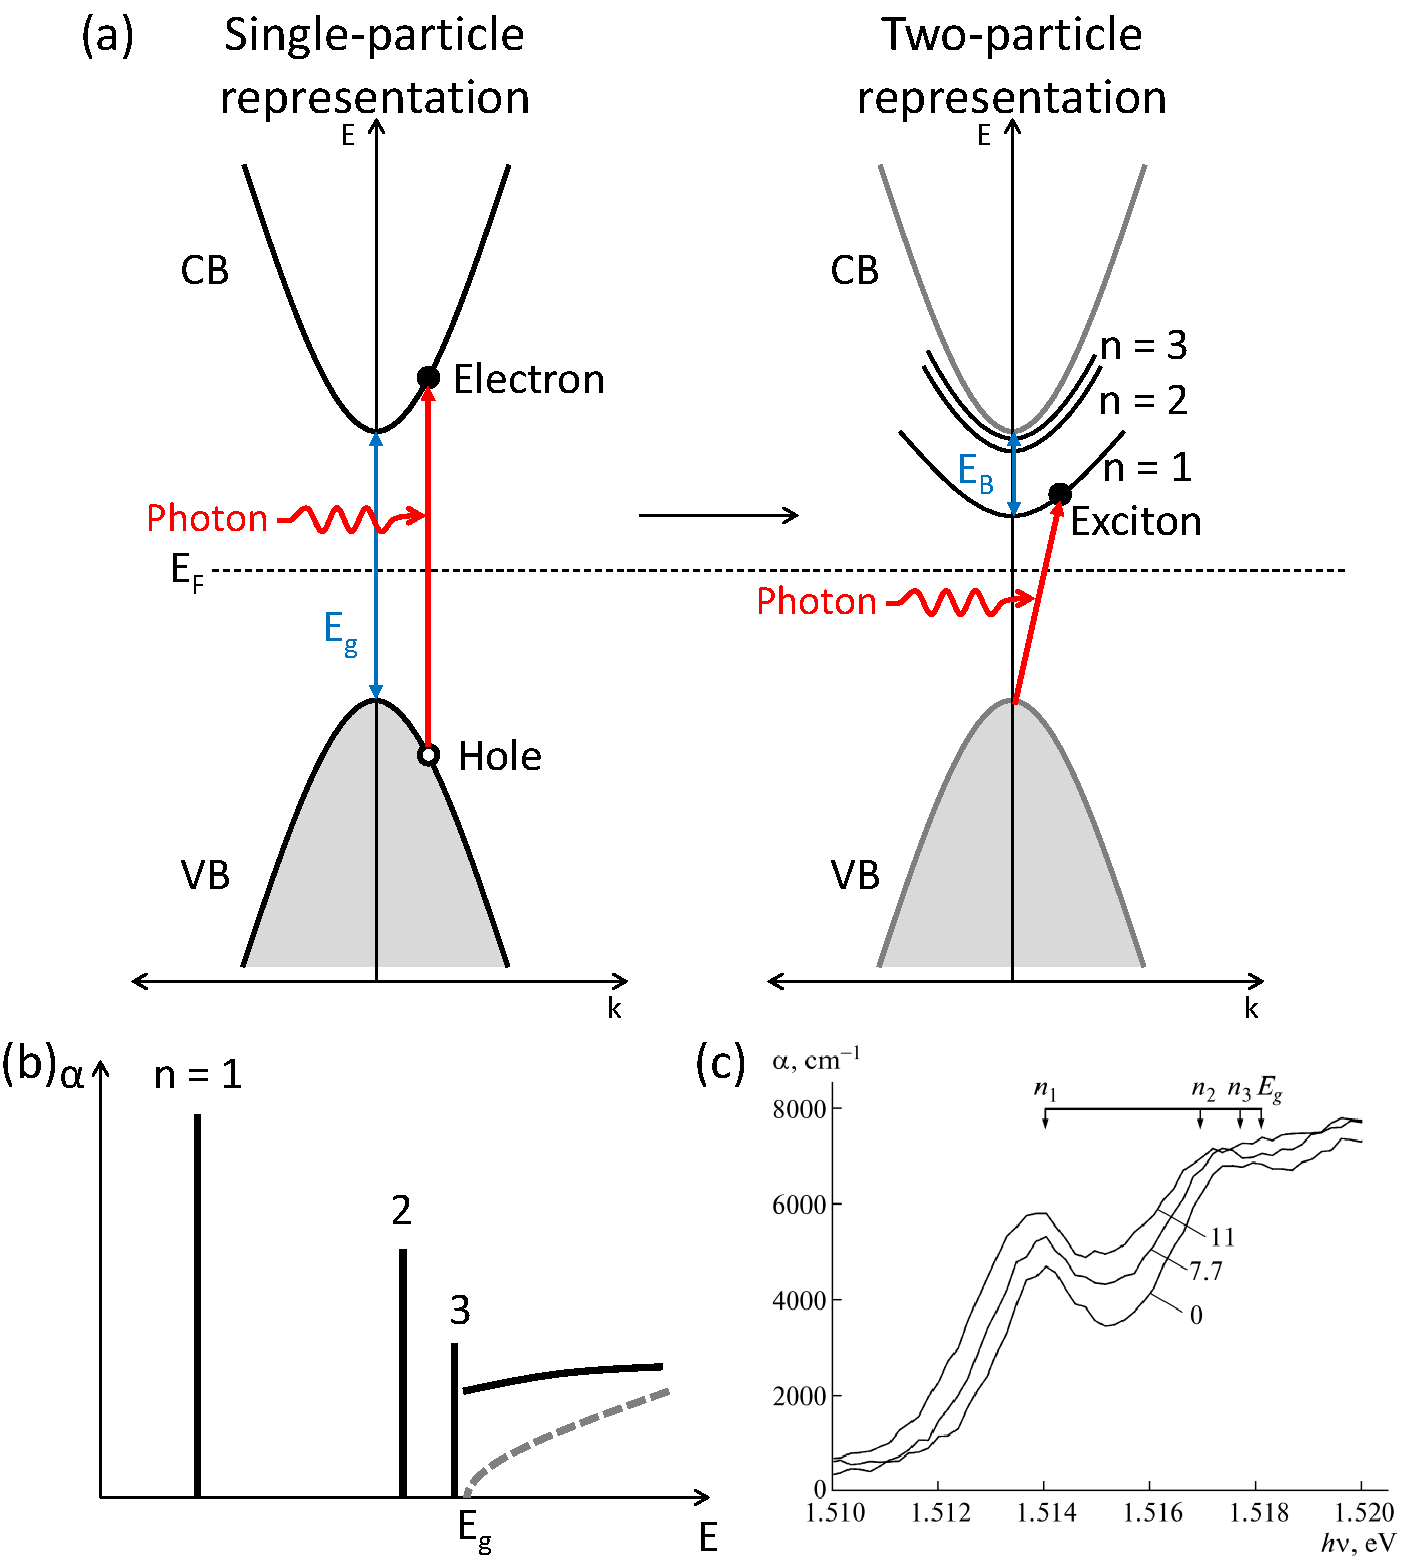
\includegraphics[width=\textwidth]{Fig1}
\caption{(a) (Left) Band structure of a semiconductor, showing the single-particle representation of the excitation of an electron-hole pair via photon absorption. (Right) Two-particle representation of the same system, illustrating exciton energy levels below the CB. (b) Theoretical absorption spectrum of a 3D semiconductor according to Eq.\,\ref{exabs} (not to scale). The dotted line shows the expected band edge absorption without the Sommerfeld factor (see text). (c) Experimental absorption spectrum of GaAs crystal at 1.7\,K, where the excitation power is labelled (W/cm$^2$). Reproduced from Ref.\,\cite{Vaganov2013}.}
\label{2Fig1}
\end{figure}
The attraction between an excited electron and hole binds them together to form a hydrogen-like neutral particle in the crystal. We can therefore use results from the hydrogen atom to find the binding energy $E_B$ and Bohr radius $a_B$ of an exciton:
\begin{subequations}
\label{ex3D}
\begin{align}
E_B &=\frac{\mu e^4}{32\pi^2\epsilon^2\epsilon_0^2\hbar^2n^2} = \frac{R_H}{n^2}\frac{\mu}{\epsilon^2 m_e} \label{exbinding3D}\\
a_B &= \frac{4\pi\epsilon\epsilon_0\hbar^2}{\mu e^4}=a_0\frac{\epsilon m_e}{\mu} \label{exrad3D},
\end{align}
\end{subequations}
where $\mu = (\frac{1}{m_e}+\frac{1}{m_h})^{-1}$ is the effective mass of the exciton, $\epsilon$ is the dielectric constant of the material, and $n$ is the energy level of the exciton ($n=1, 2, 3...$). The Rydberg constant $R_H=13.6$\,eV, and the most probably distance between a proton and electron in the ground state $a_0=0.5$\,\AA\, are defined for the hydrogen atom. Thus a series of exciton energy levels are formed below the lower edge of the CB [Fig.\,\ref{2Fig1}(a)], and the energy of an exciton $E_{ex}$ is given by
\begin{equation}
\centering
E_{ex} = E_g - E_B + \frac{\hbar^2}{2M}(k_x^2+k_y^2+k_z^2),
\label{exenergy}
\end{equation}
where $M = m_e+m_h$ is the total mass of the exciton, and the $k_i$ terms describe its motion in 3D. Eq.\,\ref{exenergy} gives the energy of free excitons that are able to move throughout the crystal, however excitons can be bound to impurities, further lowering their energy.

In inorganic materials, high $\epsilon$ gives rise to $E_B \sim 10$\,meV and $a_B \sim 100$\,\AA, and the so-called Mott-Wannier excitons extend over many unit cells, however due to low $E_B$ the effects can only be observed at low temperature. Conversely organic materials have lower $\epsilon$, such that $E_B \sim 1$\,eV and $a_B \sim 10$\,\AA. These Frenkel excitons are limited to a few unit cells, or one molecule in the case of molecular semiconductors.

Excitons can be created optically by the absorption of photons [Fig.\,\ref{2Fig1}(a)]. In bulk semiconductors, the absorption coefficient $\alpha$ of an exciton depends on the initial ground state $\ket{i}$ (filled VB and empty CB) and final state $\ket{f}$ (one promoted electron), such that
\begin{equation}
\centering
\alpha = \left| \Braket{f | i} \right|^2 \rho(E) ,
\label{exabs}
\end{equation}
where the matrix element $\braket{f | i}$ gives rise to selection rules of possible electronic transitions, and the joint density of states $\rho(E)$ is the number of states per unit energy range between the CB and VB at the photon energy $E$. In 3D $\rho(E)$ has a $\sqrt{E-E_g}$ dependence, however Coulomb interactions lead to an enhancement in the absorption by the Sommerfeld factor, and $\alpha$ is not discontinuous to zero at $E_g$ as expected from Eq.\,\ref{exabs} \cite{Bassu1997}. The theoretical absorption spectrum shown in Fig.\,\ref{2Fig1}(b), with discrete exciton lines decreasing in intensity as $n^{-3}$ \cite{Bassu1997}, and continuous absorption at higher energy due to interband transitions. Experimental data for the absorption of a GaAs crystal at 1.7\,K [Fig.\,\ref{2Fig1}(c)] shows overlap between exciton lines and band edge absorption as a result of the finite exciton peak width $\Gamma_{ex}$. The exciton linewidth is due to a number of factors: firstly homogeneous variables that affect each exciton equally, such as the radiative lifetime of the exciton $\tau_{ex} = \frac{1}{\Gamma_{ex}(0)}$ and collisions with phonons; secondly inhomogeneous factors such as impurities ($\Gamma_{imp}$), whose effects are more localised. Overall this leads to a measured linewidth $\Gamma_{ex}$ that varies with temperature $T$ as
\begin{equation}
\centering
\Gamma_{ex}(T) = \Gamma_{ex}(0) +  \Gamma_{imp}(T) +A_{ac}T + \frac{B_{op}}{\exp{\frac{\hbar\omega_p}{k_B T}}-1},
\label{exwidth}
\end{equation}
where the contribution to phonon collision has been further separated into coupling with acoustic phonons ($A_{ac}$), and interactions with polarised optical phonons of energy $\hbar\omega_p$ \cite{Dammak2009}. 

Once excitons are created, they can annihilate and emit energy in the form of photons. The formation of the charged constituents in excitons causes deformation of the crystal, and as a result of this structural rearrangement the exciton emission is redshifted with respect to absorption, known as the Stokes shift. In general Frenkel excitons in organic semiconductors show larger Stokes shifts as molecules are more easily deformable.

Observations of excitons in optical spectra depends on the coupling between excitons and photons, so exciton peak strength is partly determined by the oscillator strength $f$, given by the matrix element between the exciton and photon wavefunctions. Coupled exciton-photon states are known as exciton-polaritons. Non-propagating solutions give rise to longitudinal excitons with frequency $\omega_L$, while travelling solutions produce transverse excitons with frequency $\omega_T$. The longitudinal-transverse splitting $\omega_{LT} = \omega_L - \omega_T$ is again related to the coupling between excitons and photons, with $f \sim \sqrt{\epsilon_B} \omega_{LT}$, where $\epsilon_B$ is the background dielectric constant of the material without excitonic contributions.

\section{Excitons in 2D systems}
\label{sec:ex2D}
Exciton motion can be confined to 2D in quantum well (QW) systems, where a well material is sandwiched between barrier layers with higher $E_g$. If the well and barrier layers are periodically arranged then a multiple quantum well (MQW) or superlattice is formed. Four types of band alignment can be achieved [Fig.\,\ref{2Fig2}(a)]: in type I structures potential steps appear in both the VB and CB, thus confining both electrons and holes to the well region. In type II QWs band edges of the barrier layers are shifted in one direction with respect to the well, creating a staggered band alignment where the electrons are confined to the well and holes to the barrier region. In the most extreme case the barrier VB is above the well CB, creating a type II broken-gap arrangement. Type III QWs occur when a semimetal (with a small overlap between the VB and CB) is used as the well. For the rest of this section only type I QWs will be considered.

Type I QWs can be formed from many III-V composite materials, for example GaAs/AlGaAs, GaAs/AlAs or GaAs/GaP. In designing a QW system, one must consider the lattice constants of the materials in question as well as the electronic band structure. A large lattice mismatch will cause strain in the layers, and the growth will not be epitaxial, i.\,e.\, there will not be a well-defined crystal structure throughout the layer. The AlAs/GaAs system has good lattice matching, or alternatively a ternary alloy can be used to reach the lattice constant needed. It is also possible to use materials that can adapt to the local lattice constant up to a critical thickness despite strain. In general these inorganic QWs are grown atomically layer-by-layer, either using molecular beam epitaxy (MBE) or metalorganic chemical vapour deposition (MOCVD), where the relevant atoms are deposited onto the substrate either in the gas phase or via a molecular beam. The stoichiometric mix of relevant atoms must be carefully controlled during fabrication to create the correct structures. 

The layered structure of a QW confines carrier motion in the direction of layer growth, thus creating a 2D system. If the width of the well layer $L$ is on the order of the electron de Broglie wavelength ($\sim10$\,nm), then then carriers are essentially trapped in a finite potential well and we observe wave-like effects such as the creation of discrete energy levels in which electrons/holes can reside. Using the results for a particle in an infinite well for simplicity, the energy $E_u$ of allowed states are
\begin{equation}
\centering
E_u = \frac{\hbar^2}{2m} \left(\frac{u\pi}{L}\right)^2 ,
\label{particleboxenergy}
\end{equation}
where $m$ the mass of the carrier, and the index $u$ labels the energy level. Instead of the VB/CB, we find instead a series of minibands with different energies [Fig.\,\ref{2Fig2}(b)]. The absorption spectrum of QW systems can still be calculated using Eq.\,\ref{exabs}, however the orthogonality of eigenstates means that transitions from state $\Ket{u_1}$ in the VB to $\Ket{u_2}$ in the CB are only allowed if $u_2-u_1=0$. The joint density of states $\rho(E)$ is step-like in 2D, again with the Sommerfeld factor enhancing absorption [Fig.\,\ref{2Fig2}(c)].
\begin{figure}[h!] 
\centering    
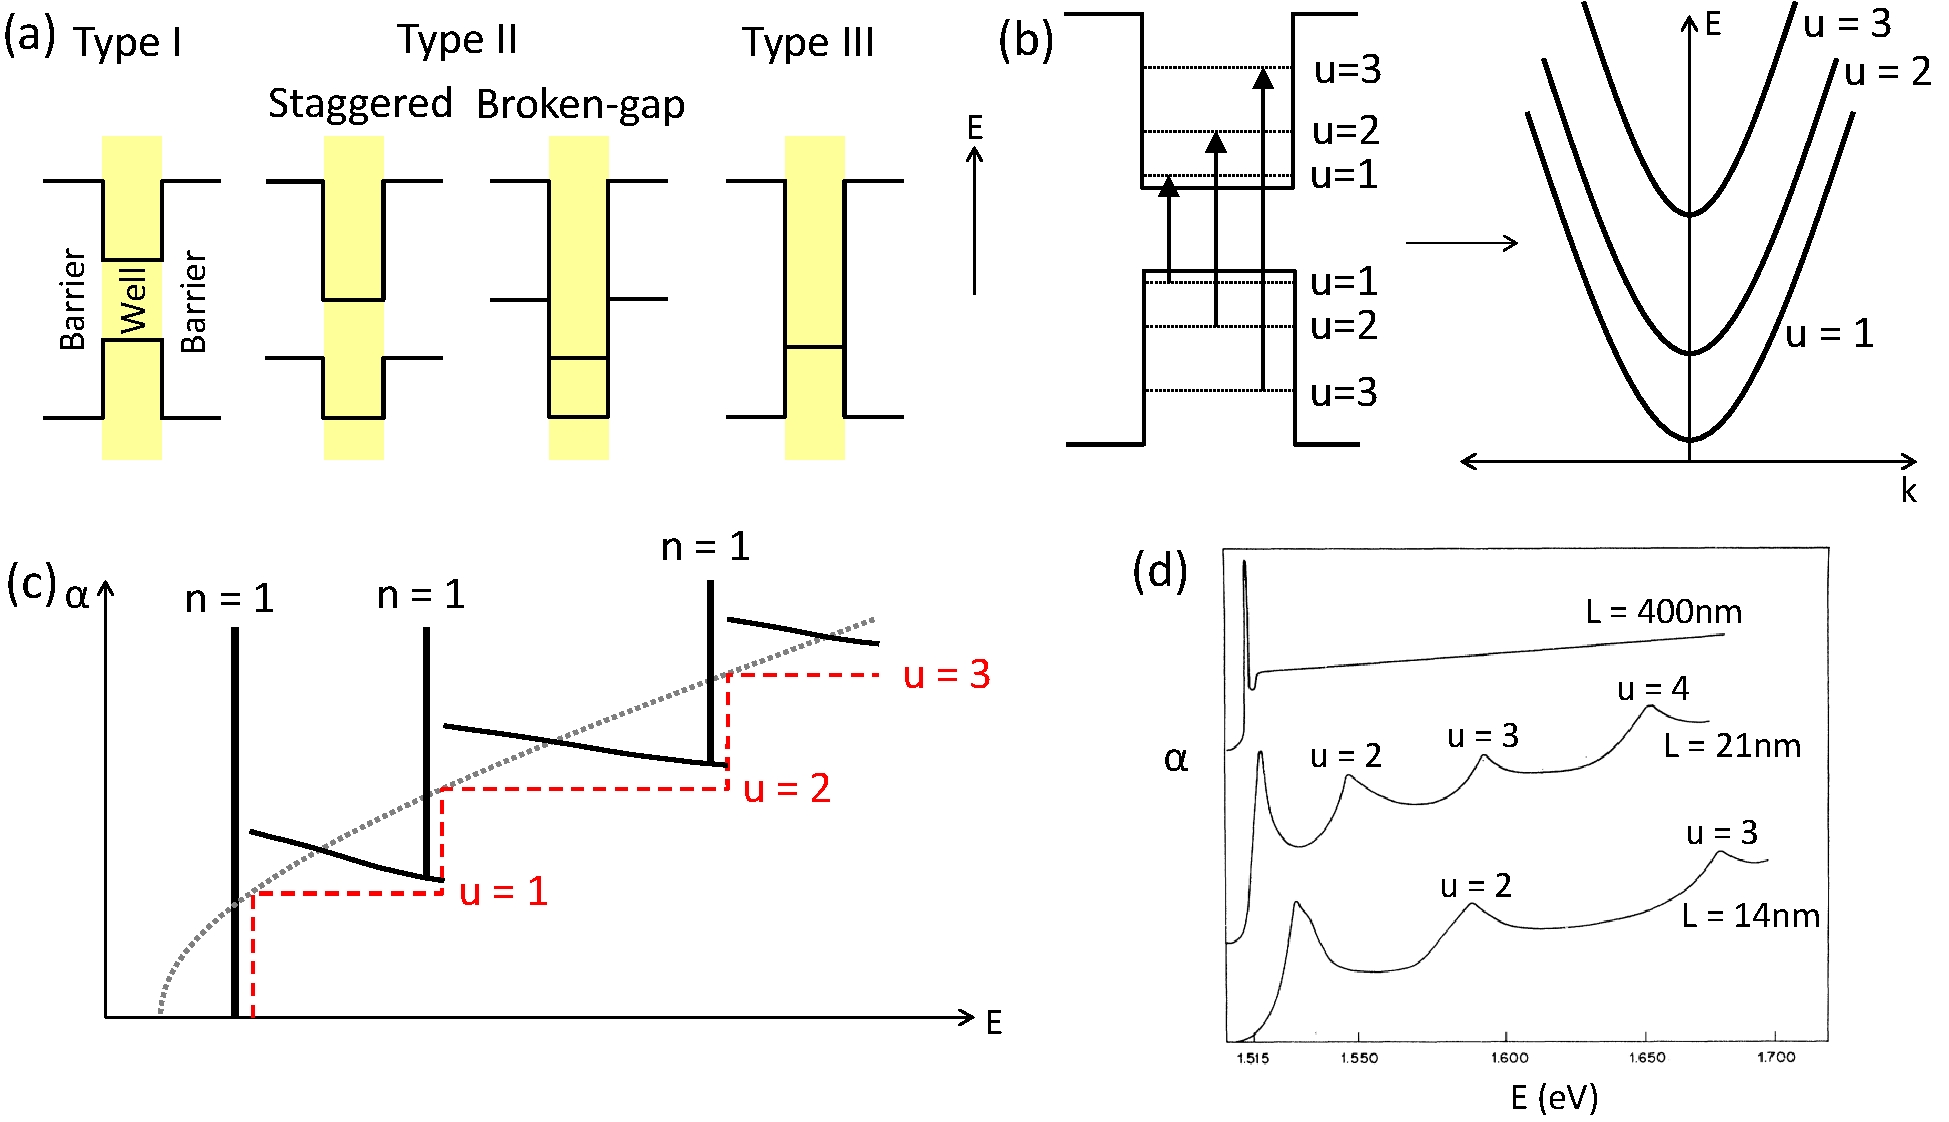
\includegraphics[width=0.53\textwidth]{Fig2}
\caption{(a) Schematic of quantum well band alignments. (b) Allowed transitions for electrons in a quantum well (left) and the resultant miniband structure (right). (c) Theoretical absorption spectrum of a 2D quantum well according to Eq.\,\ref{exabs} (black lines). The band edge absorption in 3D (grey dotted line) and 2D (red dashed line) are both shown with the Sommerfeld factor. (d) Experimental absorption spectrum of GaAs/Al$_{0.2}$Ga$_{0.2}$As quantum wells with the labelled well width $L$ at 2\,K. Only the $n=1$ exciton peaks (labelled ex) are observed, but the minibands $u$ are labelled. Adapted from Ref.\,\cite{Dingle1974}.}
\label{2Fig2}
\end{figure}

Exciton bands exist below each of the minibands, and in order to find $E_B$ we use the results for a hydrogen atom in 2D, such that
\begin{equation}
\centering
E_B =\frac{\mu e^4}{32\pi^2\epsilon^2\epsilon_0^2\hbar^2\left(n+\frac{1}{2}\right)^2} = \frac{R_H}{\left(n+\frac{1}{2}\right)^2}\frac{\mu}{\epsilon^2 m_e} .
\label{exbinding2D}
\end{equation}
Therefore the energy of the exciton bands $E_{ex}$ can be described by
\begin{equation}
\centering
E_{ex} = \Delta E_u - E_B + \frac{\hbar^2}{2M}(k_x^2+k_y^2) ,
\label{exenergy2D}
\end{equation}
where $\Delta E_u$ describes the transition between energy levels $u$ in the CB and VB. The expected absorption spectrum of a QW structure is shown in Fig.\,\ref{2Fig2}(c), while experimentally measured spectra for GaAs/Al$_{0.2}$Ga$_{0.8}$As QWs are shown in Fig.\,\ref{2Fig2}(d). Note how the change in $L$ affects the allowed $\Delta E_u$, with $L=400$\,nm essentially appearing as a 3D system.

We can see from Eq.\,\ref{exbinding2D} that the reduction in dimensionality leads to a factor of 4 enhancement in $E_B$ for the $n=1$ state, so exciton effects should be observable at higher temperatures in QWs. Similarly $a_B$ is reduced by a factor of 2 in QWs as a result of confinement. For this reason is it often said that excitonic effects are stronger in QWs, with increased overlap between the electron and hole wavefunctions.

\section{Properties of PbI perovskites}
%Organic-inorganic metal halide perovskite semiconductors can combine the distinct properties of its organic (ease of processing, structural diversity, plastic mechanical properties) and inorganic (band structure variability, electrical mobility, thermal and mechanical stability) constituents into one composite.
\subsection{Structure and bonding}
Metal halide \ce{RNH3MZ3} organic-inorganic semiconductors are based on the \ce{ABX3} perovskite crystal structure [Fig.\,\ref{2Fig3}(a)], consisting of a corner-sharing octahedra network of halogen atoms Z (most commonly I, Br or Cl) with a metal atom M in the centre of each octahedron (\ce{+2} valence metals such as Pb, Sn, Cd, Zn, Cu, or Co). Organic mono-ammonium molecules \ce{RNH3} hydrogen bond to halogen atoms and reside in the interstices between octahedra [Fig.\,\ref{2Fig3}(b)], and as a result only very short molecules are used, the most common of which is \ce{CH3NH3}. The band gaps of such semiconductors can be engineered by changing the metal and halogen composition, and recently lead halide-based semiconductors have been used as a light absorbing layer in solar cells, producing efficiencies of up to 16\%, and there is currently a drive to find lead-free alternatives for wider use \cite{Lee2012, Heo2013, Liu2013, Hao2014}. A change in the stoichiometric mix of organic and inorganic constituents results in the formation of lower dimension structures, for example 2D layered systems, or 1D inorganic wires \cite{Nagami1996, Fukumoto2000, Fujisawa2004, Pradeesh2010}. From here we will focus on <100> oriented 2D lead iodide (PbI) perovskites \cite{Mitzi2001}.

The self-assembled structure of 2D hybrid PbI perovskites with formula \ce{(RNH3)2PbI4} are shown in Fig.\,\ref{2Fig3}(c), and consist of alternating layers of corner-sharing \ce{PbI6} octahedra and interdigitating \ce{RNH3} molecules (where R is an organic moiety). The organic molecules have larger $E_g$ (\sim6$\,eV) than the inorganic layers ($\sim3$\,eV), and form a type I MQW structure \cite{Ishihara1994, Pradeesh2009b}. The width of the QW (PbI octahedra) is $\sim6.5$\,\AA~\cite{Ishihara1989}. The bonding in inorganic layers is primarily ionic as Pb-I distances are more comparable to the sum of ionic radii \cite{Mousdis2000}. Inorganic sheets are sandwiched between layers of organic molecules via hydrogen bonding between $\textrm{NH}_3$ groups and I atoms, while the van der Waals or aromatic-aromatic interactions that bind organic molecules together can (de)stabilise the perovskite structure \cite{Mitzi2001a}. Like other layered materials such as graphene or transition metal dichalcogenides, it is possible to break these van der Waals bonds and cleave the structure and produce thinner samples.
\begin{figure}[h!] 
\centering    
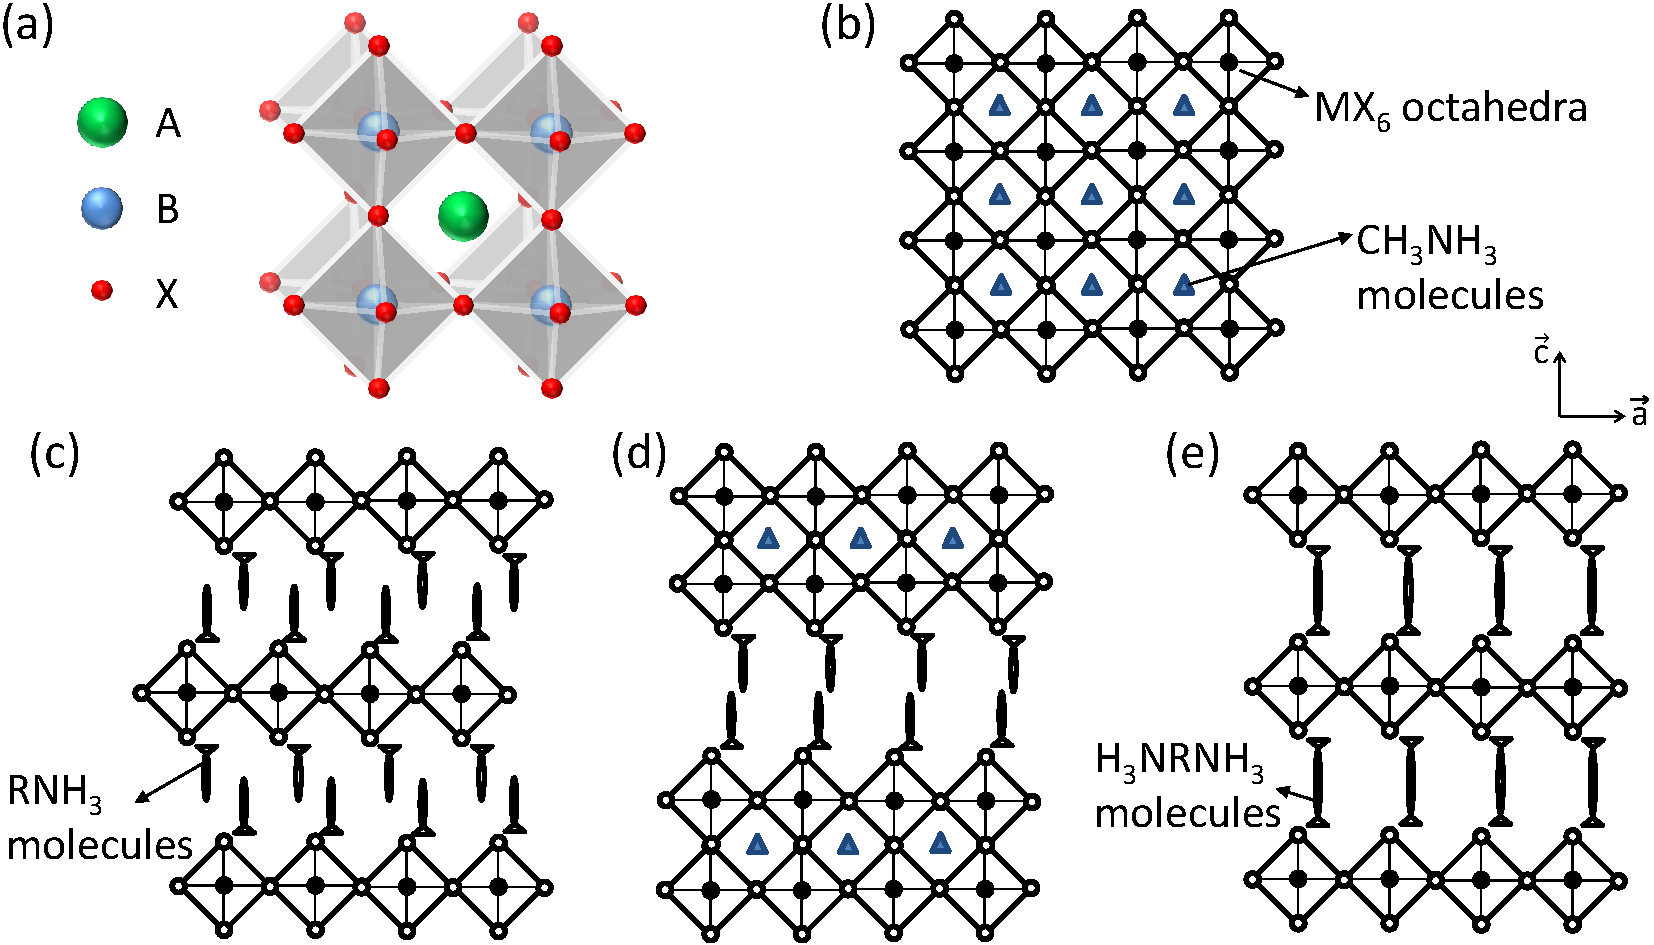
\includegraphics[width=\textwidth]{Fig3}
\caption{Crystal structure of (a) \ce{ABX3} perovskite, (b) 3D perovskite \ce{(CH3NH3)PbI3}, (c) 2D perovskite \ce{(RNH3)2PbI4}, (d) 2D multilayered perovskite \ce{(RNH3)2(CH3NH3)Pb2I7}, and (e) 2D diammonium perovskite \ce{(H3NRNH3)PbI4} viewed along the crystallographic $\vec{B}$ axis.}
\label{2Fig3}
\end{figure}

There are two main orientations for consecutive inorganic layers: eclipsed layers produce a monoclinic structure, while staggered layers produce an orthorhombic structure \cite{Billing2006}. The orientation is chosen to accommodate organic molecules in the structure. Phase transitions from the orthorhombic phase to the monoclinic phase will lead to a halving of the $c$ lattice parameter due to increased symmetry \cite{Billing2008}.

There are only a few limits on the organic molecule \ce{R} in the structure. The cross section of the molecule should be small enough to fit into the interlayer space between four adjacent octahedra ($\lesssim 40$\,\AA$^2$) \cite{Mitzi2001a}. However their lengths are not constrained so long as the intermolecular forces are strong enough to hold the structure together. Systems with aromatic molecules tend to be better organised with more crystallinity since such molecules allow for self-assembly using stronger aromatic-aromatic interactions, conversely large organic groups will hinder self assembly and reduce crystallinity \cite{Zhang2009}. In general very simple organic molecules are used, for example those based on simple alkane chains (($\textnormal{C}_n\textnormal{H}_{2n+1}$\ce{NH3)2PbI4}, C$_n$PI hereafter), ring structures (\ce{(C6H9NH3)2PbI4}, CHPI), or aromatic molecules (\ce{(C6H5C2H4NH3)2PbI4}, PAPI). However more complex organic molecules can be incorporated, for example optically active ligands \cite{Billing2006, Teshima2003} and fullerene derivatives \cite{Kikuchi2005, Kawabata2009}. 

The basic 2D layered structure can be varied in a series of ways. For instance the width of QWs	can be varied by extending the inorganic sheets to contain multiple layers of \ce{PbI6} octahedra (\ce{(RNH3)2(CH3NH3)}$_{n-1}\textnormal{Pb}_n\textnormal{I}_{3n+1}$) [Fig.\,\ref{2Fig3}(d)] \cite{Calabrese1991}. Another is with the use of diammonium organic molecules, which can hydrogen bond to two consecutive inorganic layers, therefore eliminating the need for van der Waals interactions between the interweaving molecules (\ce{(H3NRNH3)PbI4}) [Fig.\,\ref{2Fig3}(e)].

\subsubsection{Phase transitions in $\textrm{C}_n$PI}
\label{sec:Cnphases}
Four main phases of $\textrm{C}_n$PI perovskites have been identified. For temperatures $< -30^{\circ}$C (phase I), the crystal exhibits twinning so atomic positions cannot be determined. Between $-30$ and $15^{\circ}$C  (phase II), organic chains are ordered with uniform tilting angle. The structure then undergoes a pre-melting transition, leading to dynamic rotational disorder of $\textrm{NH}_3$ groups and a small decrease in the lattice parameter $c$ \cite{Barman2003}. Between $\sim 15$ and $65^{\circ}$C (phase III), organic chains show much more conformational disorder and become tilted at different angles, leading to a large increase in $c$, and thus an increase in volume since no lateral motion occurs \cite{Barman2003}. Above $65^{\circ}$C (phase IV), organic chains appear to be `melting' \cite{Ishihara1990, Xu1991, Ishihara1989}. Simulations show that after the melting transition alkyl chains are no longer all-trans, and the introduction of gauche defects leads to a shortening of the chain and an increase in its effective cross-sectional area. Conflicting demands of close packing that optimise dispersive interactions and the larger area required by conformationally disordered chains can no longer be met by a uniformly tilting arrangement, and the non-uniform tilt allows for increased space for individual chains \cite{Naik2010}. Changes in conformation during phase transitions also cause a spatial shift in the coupling between $\textrm{NH}_3$ groups and inorganic octahedra \cite{Pradeesh2009}. In order to accommodate the changes in alkyl chains, $\textrm{PbI}_6$ octahedra can undergo two types of structural change: they can tilt perpendicular or parallel to the inorganic sheets. During perpendicular tilting octahedra are tilted with respect to each other, whereas parallel tilting leads to an overall corrugation of inorganic layers \cite{Billing2008}. For $\textrm{C}_{12}$-, $\textrm{C}_{14}$-, $\textrm{C}_{16}$-, and $\textrm{C}_{18}$PI phase III is orthorhombic with staggered inorganic sheets, and phase IV is monoclinic with eclipsed inorganic sheets \cite{Billing2008}.    
%\begin{figure} [h!]
%\centering
%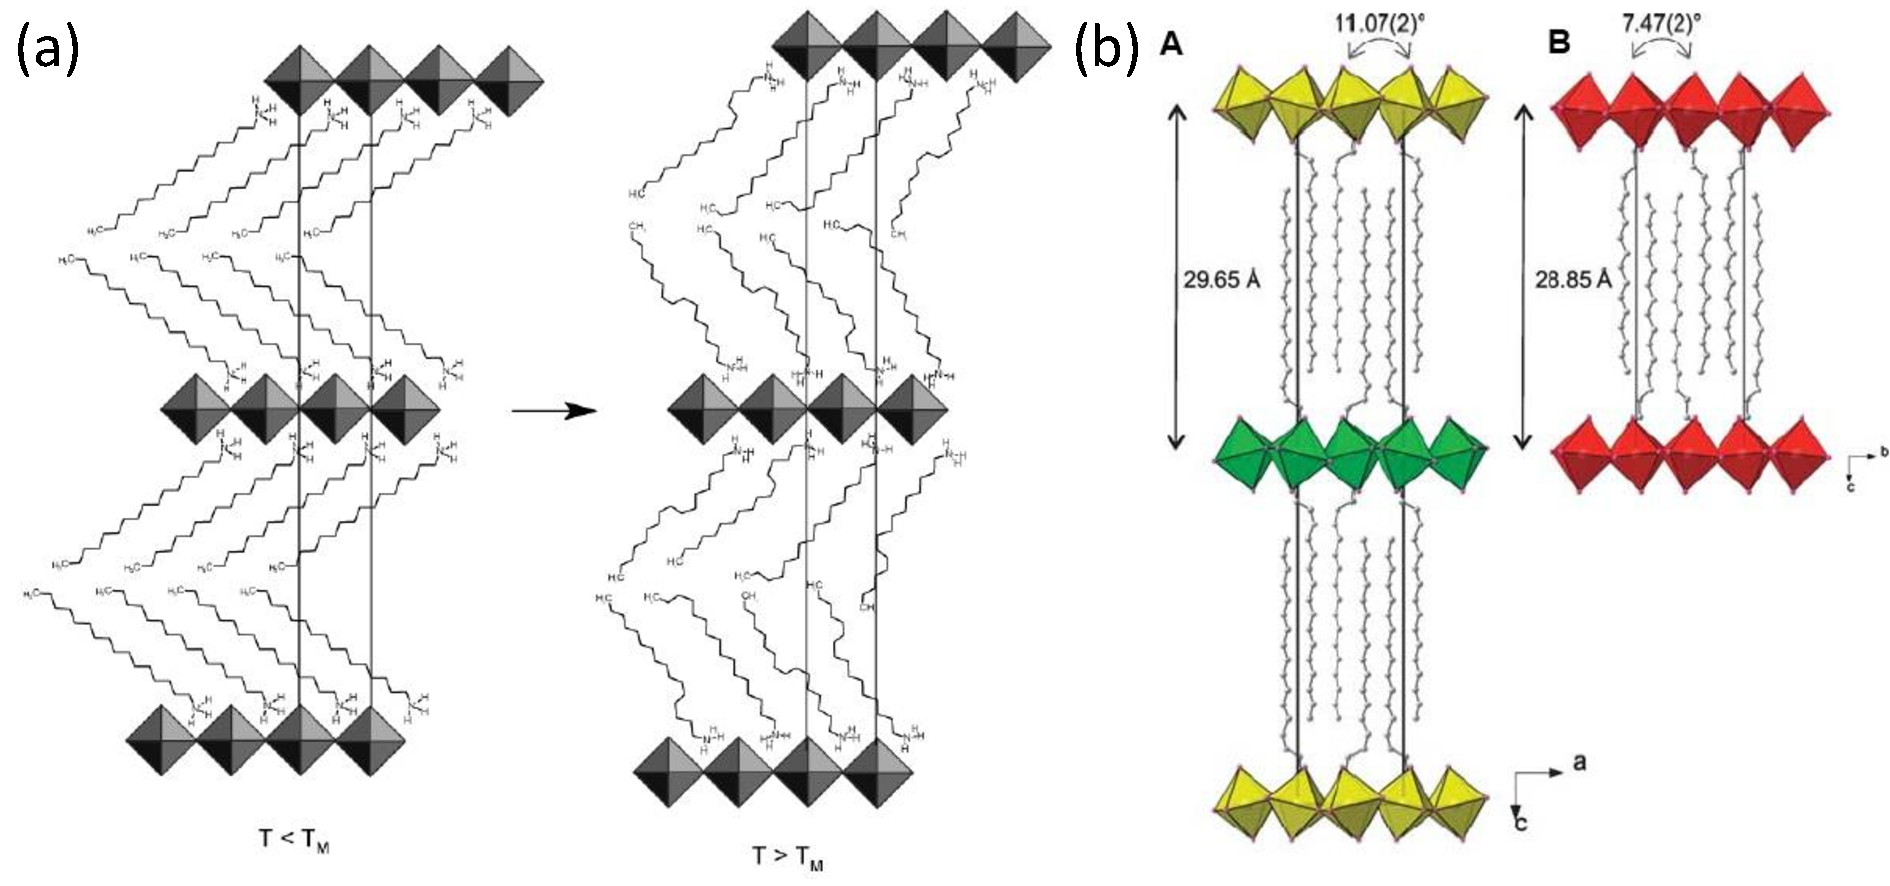
\includegraphics[width=\textwidth]{Fig4}
%\caption {(a) Structure of $\textrm{C}_{n}$PI ($n$=12, 14, 16, 18) before (A) and after (B) the pre-melt transition. A is orthorhombic, and B is monoclinic so the lattice parameter $c$ is halved. (b) Schematic of the melting transition in $\textrm{C}_{10}$PI. Below the melting temperature $T_M$, the chains adopt an all-trans conformation (no gauche defects \cite{Naik2010}) with a well defined tilt angle of around $55^{\circ}$ \cite{Venkataraman2002, Venkataraman2002a}. Above $T_M$, alkylammonium chains are conformationally disordered with different tilt angles. (a) Reproduced from Ref.\ \cite{Billing2008}, (b) from \cite{Barman2003}.}
%\label{2Fig4}
%\end{figure}

The switching between orthorhombic and monoclinic phases can be controlled by parameters other than temperature. Pradeesh \textit{et al.}\ showed that the phases present in spin coated films of $\textrm{C}_{12}$PI depend on the thickness of the sample, as well as ageing effects. They postulated that this is due to strain, where high strain in thicker samples favours the flatter orthorhombic phase. Ageing effects, where a sample in the monoclinic phase gradually shifted to the orthorhombic phase, can be stopped by annealing or capping with poly(methyl methacrylate) (PMMA) \cite{Pradeesh2009}.

\subsection{Fabrication and processing techniques}
\subsubsection{Silica-gel method}
An aqueous solution of Pb($\textrm{CH}_3 \textrm{COO)}_2$, $\textrm{C}_n\textrm{H}_{2n+1}\textrm{NH}_2$, $\textrm{CH}_3$COOH, and $\textrm{Na}_2\textrm{SiO}_3$ is prepared in a test tube, and becomes a gel after approximately one week. At this point an aqueous solution of KI is poured into the gel and the $\textrm{I}^-$ ions diffuse slowly into the gel to form $\textrm{C}_n$PI single crystals. About a month after the introduction of KI, platelet-like crystals form, approximately $2\times 2\times 0.1$~mm in size. However crystals for perovskites where $n=4,6$ cannot be produced using this method \cite{Ishihara1990}.

The silica-gel method allows multiple components to be mixed in solution on a nanometre scale, which can produce very homogeneous materials. The technique can also be used to make thin films by dissolving the raw ingredients in a suitable solvent (e.\,g.\,an alcohol) that is fast gelling and drying. The necessary condensation reaction and solvent evaporation will take place after the solution is applied to a substrate, leaving behind a wet gel film that can be heated to produce a dry film, but in order to avoid cracking the wet film should generally be less than 1\,$\mu$m thick. Thin gel films are usually amorphous, but surfactants on the substrate can help with assembly and annealed films are generally crystalline \cite{Mitzi2001b}.

\subsubsection{Solution crystal growth}
\label{sec:solutiongrowth}
The silica-gel method is time intensive, therefore crystals of a similar or larger size are more commonly produced from solution. Pb$\textrm{I}_2$, R$\textrm{NH}_2$ and HI are usually mixed in stoichiometry and left for solvent evaporation \cite{Kitazawa1996, Tang2001, Ishihara1994}. The basic reaction scheme is \ce{2RNH3 + 2HI + PbI2 -> (RNH3)2PbI4}. After around one week single crystals form, although the rate of evaporation can be controlled to change the morphology of crystals \cite{Cheng2010}. The difficulty lies in finding solvents that will dissolve both the inorganic and organic parts of the perovskites, and examples include acetone \cite{Hong1992}, dimethylformamide (DMF) \cite{Kitazawa1996}, and HI \cite{Barman2003}. If the evaporation is less controlled, this method can be used to create perovskite powder, which can later be dissolved in a suitable solvent and used in spin coating.

\subsubsection {Spray pyrolysis/drying}
Spray pyrolysis produces particles when misted streams of precursor solution are introduced to a furnace. Multicomponent particles can be prepared due to microscale reactions inside the micrometre-sized droplets, and new phases with narrow size distributions and non-agglomeration can be obtained rapidly after solvent evaporation and as a result of high temperature and inert gas streams inside the furnace reactor \cite{Cheng2005}. 

A precursor solution of stoichiometric quantities of $\textrm{PBI}_2$ and $\textrm{C}_6\textrm{H}_5\textrm{C}_2\textrm{H}_4\textrm{NH}_3\cdot\textrm{HI}$ in tetrahydrofuran (THF) is used to prepare PAPI powder. From scanning electron microscope (SEM) images the powder particles are $\sim 1\, \mu$m in size, however XRD data indicate the structure is less organised than PAPI prepared by other methods, e.\,g.\, spin coating. The photoluminescence (PL) spectrum of PAPI powder shows a strong exciton peak, indicating the formation of the required layered structure, however the wavelength is shifted by around 5\,nm, likely due to distortion of PbI sheets \cite{Cheng2005}.

A similar technique of spray drying can be used to produce perovskite nanoparticles. The precursor solution is prepared by bubbling a flow of dry HI into a dry ethereal solution of organic amine. Drying droplets (initial mean diameter $\sim 35\,\mu$m) are carried from the aerosol generator by dry air into an evaporation chamber at $250^{\circ}$C. Dried nanoparticles created using this method are mostly spherical, but with a large size distribution ($50-500$\,nm diameter; average $60\pm10$\,nm). The perovskite crystallises at the edge of the particle while the centre is depleted, therefore larger nanoparticles are hollow, while smaller particles are denser due to their fast drying rate. XRD data indicate the nanoparticles are crystalline, with a small redshift of a few nanometres in exciton PL caused by strain. The nanoparticles are also fairly photo-stable, with a drop in PL intensity of around 30-50\% after illumination of 1\,hour \cite{Audebert2009a}.

\subsubsection {Langmuir-Blodgett technique}
The Langmuir-Blodgett (LB) technique uses a movable barrier to apply pressure to a monolayer of molecules at a liquid-gas interface. When molecules are close enough van der Waals forces can create close packing, thus forming a thin film [Fig.\,\ref{2Fig6}(a)] \cite{Mitzi2001b}. Era \textit{et al.}\ used LB to create thin films of $(\textrm{C}_{22}\textrm{H}_{45}\textrm{NH}_3)_2\textrm{PbBr}_4$. The long chain ammonium bromide ($\textrm{C}_{22}\textrm{H}_{45}\textrm{NH}_3$Br) is spread on an aqueous subphase containing Pb$\textrm{Br}_2$ and $\textrm{CH}_3\textrm{NH}_3$Br from a chloroform and DMF solution. The monolayer is then pressed to a surface pressure of 30\,mN$\textrm{m}^{-1}$, then deposited on a hydrophobidised fused quartz substrate. Layer-by-layer deposition of LB films allows control over the film thickness. Films show strong exciton absorption peaks, with linear increase in the absorption intensity for each additional layer [Fig.\,\ref{2Fig6}(b)] \cite{Era2000}.
\begin{figure} [h!]
\centering
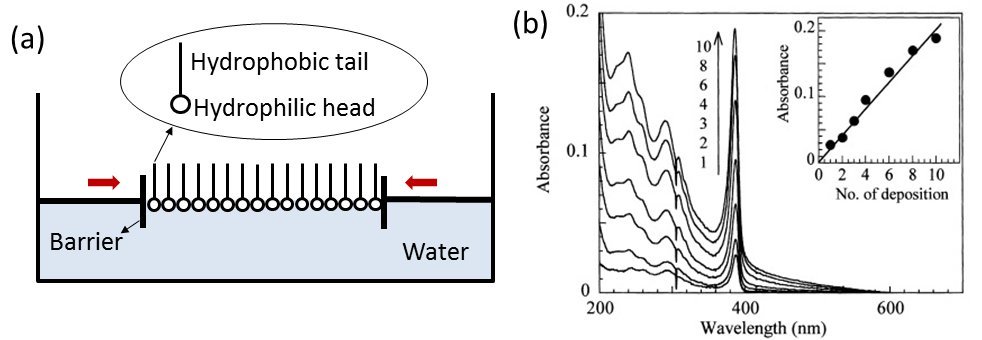
\includegraphics[width=\textwidth]{Fig6}
\caption{(a) Schematic of Langmuir-Blodgett setup and the amphiphilic nature of molecules ordered on the water-air interface. (b) Absorption spectra of LB film obtained using the labelled number of depositions, and exciton absorbance intensity against the number of depositions (inset). Reproduced from Ref.~\cite{Era2000}.}
\label{2Fig6}
\end{figure}

\subsubsection{Intercalation}
Perovskite films can be formed by the intercalation of organic molecules into an inorganic framework. Pb$\textrm{I}_2$ films are deposited onto substrates by vacuum deposition or spin coating, and a solution of organic ammonium iodide prepared. The Pb$\textrm{I}_2$ covered substrates are dipped in the iodide solution and dried. The resulting films have the same properties as films created using other methods \cite{Liang1998}, and the film thickness is controlled by the initial Pb$\textrm{I}_2$ thickness. In the case of CHPI only 10\,s is needed to complete intercalation for a film $\sim70$\,nm thick \cite{Pradeesh2009a}.

A similar dipping method has been used to make thin films of diammonium \ce{(H3NC12H25NH3)PbI4}. Hydrophilic quartz substrates are alternately dipped in organic diammonium iodide and \ce{PbI2} solutions, with care taken to remove excess reactants after each step. The procedure can be repeated as needed to create multilayers of self-assembled quantum wells and control the film thickness \cite{Matsui2002}.

Gaseous intercalation has also been demonstrated by Era \textit{et al.}. A 20\,nm thick film of Pb$\textrm{I}_2$ is vacuum deposited on a quartz substrate, then exposed to vaporised organic ammonium iodide ($\textrm{C}_6\textrm{H}_5\textrm{C}_2\textrm{H}_4\textrm{NH}_3\textrm{I}$). Both XRD and absorption confirm the formation of PAPI, although in XRD signatures of Pb$\textrm{I}_2$ can still be seen \cite{Era1998}.

Recently in-situ measurements on liquid-phase intercalation has shown that the process begins from the top surface of the \ce{PbI2} film, and proceeds parallel to the $\vec{c}$ axis. Organic molecules attach to the top \ce{PbI2} layer as terminal groups, and transform the edge-sharing PbI octahedra into a corner-sharing network. Interstices are opened for the diffusion of organic molecules, which interact with the bottom surface of the same layer, thus converting the \ce{PbI2} layer into full 2D perovskite monolayer. Further diffusion continues intercalation for subsequent layers [Fig.\,\ref{2Fig7}]. This process requires a non-polar solvent that will not compete with the hydrogen bonding between the inorganic and organic constituents, and an optimum organic iodide concentration exists due to steric hindrance of neighbouring molecules \cite{Ahmad2014}.
\begin{figure} [h!]
\centering
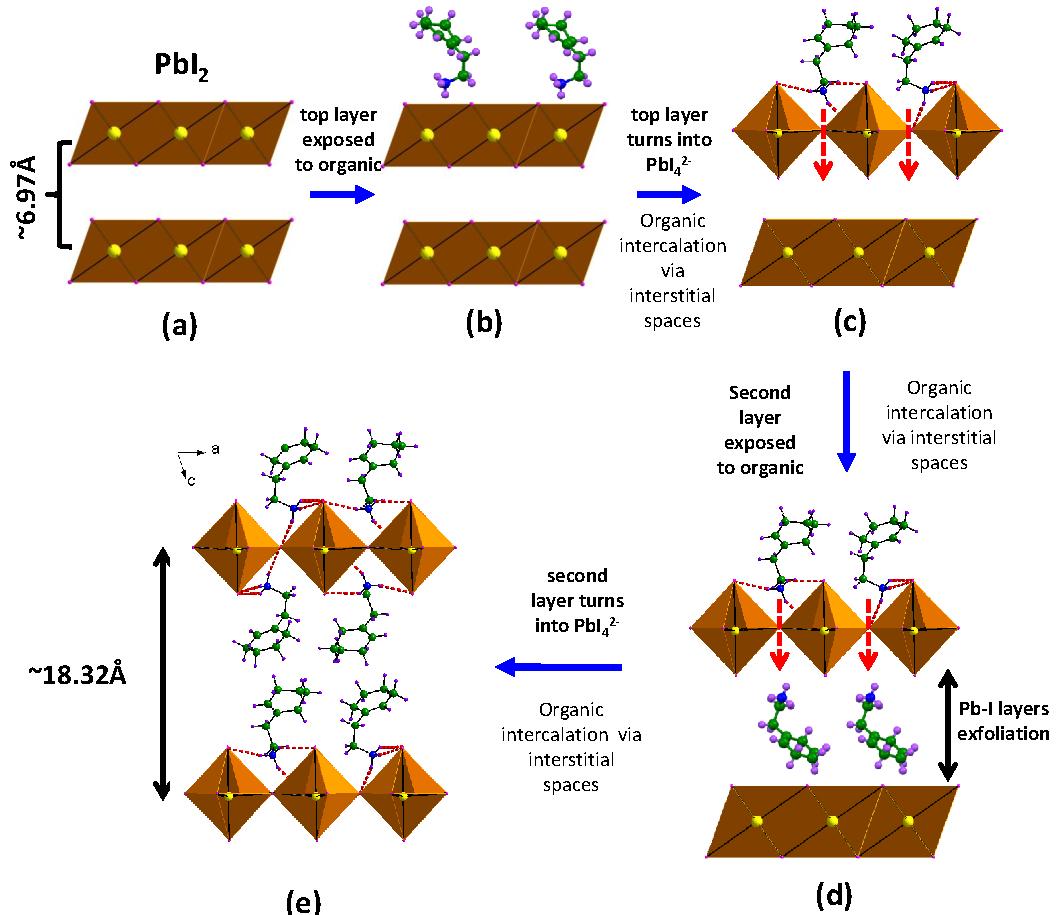
\includegraphics[width=\textwidth]{Fig7}
\caption{Molecular dynamics for the liquid-phase intercalation of organic ammonium iodide molecules into \ce{PbI2} film.}
\label{2Fig7}
\end{figure}

\subsubsection{Dual-source vacuum deposition}
PAPI films can be created using a dual-source vacuum deposition method, where both Pb$\textrm{I}_2$ and $\textrm{(C}_6\textrm{H}_9\textrm{C}_2\textrm{H}_4\textrm{NH}_3)\textrm{I}$ are deposited simultaneously on a quartz substrate. The created films show the same sharp exciton absorbance peaks as films and crystals created by other methods [Fig.\,\ref{2Fig8}], however the films are disordered as XRD data show no peaks at high $\theta$. The growth of the layered perovskite structure appears to occur in the solid phase on the substrate \cite{Era1997}. As the organic ammonium halide may dissociate into an amine and HI, care needs to be taken with choice of evaporation rates, or else films can be multiphasic, disordered or defective \cite{Mitzi1999}.
\begin{figure}[h!]
\centering
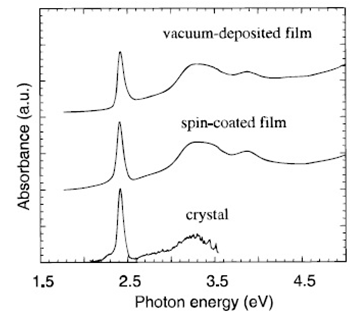
\includegraphics[width=0.6\textwidth]{Fig8}
\caption{Absorbance spectra of a vacuum deposited film, a spin coated film, and a single crystal sample of PAPI. Reproduced from Ref.\ \cite{Era1997}.}
\label{2Fig8}
\end{figure}

\subsubsection{Single source thermal ablation}
Single source thermal ablation involves the vaporisation of a material onto a substrate in order to form a film. A powder of the material is placed on a tantalum heater, the chamber is pumped to vacuum, and a current passed through the heater. The starting material is vaporised from the heater surface and reassembles on the substrate above. The important control variable is the rate at which the heater reaches its final temperature, as a low rate may lead to multiphasic or defective films. Substrates can undergo multiple ablations, and the mass of material on the heater can also be used to control film thickness \cite{Mitzi1999}. AETHPI (\ce{C18H28N2S2PbI4}) films have been created using this method. Luminescence spectra show that as-formed films have only traces of a small exciton peak, however quantum well quality is improved by annealing as the exciton peak intensity increases \cite{Chondroudis2000}.
%\begin{figure} [h!]
%\centering
%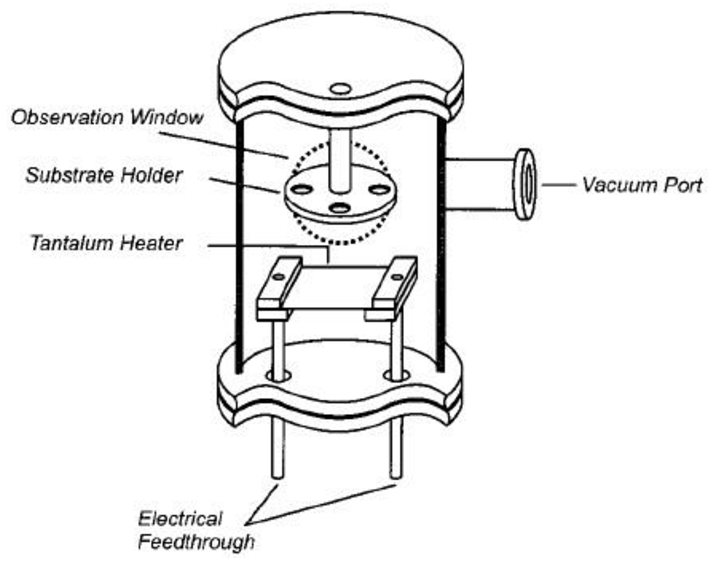
\includegraphics[width=0.7\textwidth]{Fig9}
%\caption{Cross section of single source thermal ablation apparatus. The starting material is placed on the tantalum heater, sublimates and forms a thin film on the substrate above. Reproduced from Ref.\ \cite{Chondroudis2000}.}
%\label{2Fig9}
%\end{figure}

\subsubsection{Spin coating}
Thin films can easily be produced by spin coating a perovskite solution on a substrate. Drops of solution are added to spinning substrates, and as the solvent evaporates a polycrystalline film is left behind. Suitable solvents include DMF \cite{Kikuchi2005}, THF \cite{Kataoka1994}, and acetonitrile \cite{VijayaPrakash2009}. The films produced have the same optical and electronic properties as single crystals, and the crystallographic $\vec{c}$ axis is perpendicular to the surface of the films \cite{Kataoka1993}. The films are generally smooth and can have a roughness of 1-2\,nm, although the solvent, substrate preparation, perovskite solution concentration, substrate temperature and spin speed all affect the thickness and morphology of films \cite{Mitzi2001b}. In thicker films, strain and uneven crystal planes lead to stacking imperfections, which may give rise to distorted quantum wells of differing widths and a decrease in the intensity of exciton absorption/luminescence \cite{VijayaPrakash2009}.

PbI perovskite samples tend to degrade over time due to moisture in the air, so a PMMA matrix doped with nanocrystalline PAPI can be created in order to suppress degradation \cite{Kitazawa1998}. PPMA, Pb$\textrm{I}_2$, and $\textrm{C}_6\textrm{H}_9\textrm{C}_2\textrm{H}_4\textrm{NH}_3\textrm{I}$ are dissolved in DMF then spin coated onto a glass substrate, and the resulting film annealed (thickness $\approx200$\,nm). The $\vec{c}$ axis of PAPI crystals are perpendicular to the surface of the film, and a strong exciton absorption at 2.4\,eV is seen as well as a step-like feature at 2.7\,eV due to interband transitions [Fig.\ \ref{2Fig10}(a)]. The binding energy of excitons in PMMA doped films is around 300\,meV, larger than in pure PAPI samples (250\,meV) due to dielectric confinement of PMMA. After two months in a humidity controlled box, absorption of the PAPI-doped PMMA sample is almost unchanged, however the spin coated PAPI film is degraded and no exciton peak can be seen [Fig.\,\ref{2Fig10}(b)].
\begin{figure}
\centering
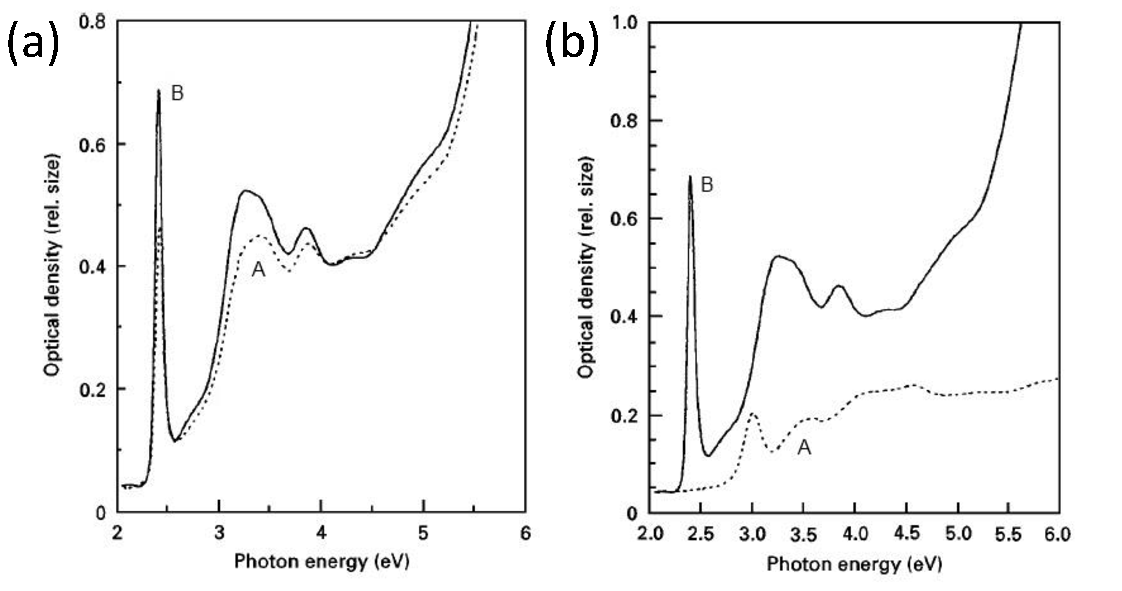
\includegraphics[width=\textwidth]{Fig10}
\caption{ (a) Absorption spectra of A) PAPI film spin coated using acetonitrile solution (dotted line), and B) PAPI doped PMMA annealed at $125^{\circ}$C for 10 minutes (solid line). (b) Absorption spectra of above films after being in a humidity controlled box for two months. Reproduced from Ref.\,\cite{Kitazawa1998}.}
\label{2Fig10}
\end{figure}

The degradation of perovskite films is partly caused by the production of halide radicals, which can form halogen gases or react with organic moieties, Structures with more electron-rich organic molecules are therefore less resistant to attack from electrophilic halide radicals \cite{Wei2014}. Kondo \textit{et al.} reported oxygen($1s$) signatures in the photoelectron spectrum of photo-irradiated PAPI films, so photo-induced oxidation is another likely mechanism for photo-degradation \cite{Kitazawa2002}.

\subsubsection{Patterning}
Patterned PAPI films have been produced using a micromoulding in capillaries method (MIMIC). Polydimethylsiloxane (PDMS) moulds are created from silicon masters, then placed in conformal contact with pre-cleaned silicon substrates so the channels of the mould formed capillaries. A solution of PAPI dissolved in DMF is dropped on one end, and the channels are spontaneously filled by capillary force [Fig.\,\ref{2Fig11}(a)]. The mould and solution are then cured for 2\,hours at $65^{\circ}$C. In general the film stripes in Fig.\ \ref{2Fig11}(b) are defect free, however some edge defects are seen in C (channel width 0.8\,$\mu$m) since the channels are more difficult to fill when the width decreases. The width of film stripes also tend to be a little smaller than the width of mould channels, and a shrinkage of around 25\% is seen after solvent evaporation.  The patterned films have same the optical properties as unpatterened films \cite{Cheng2003}.
\begin{figure} [h!]
\centering
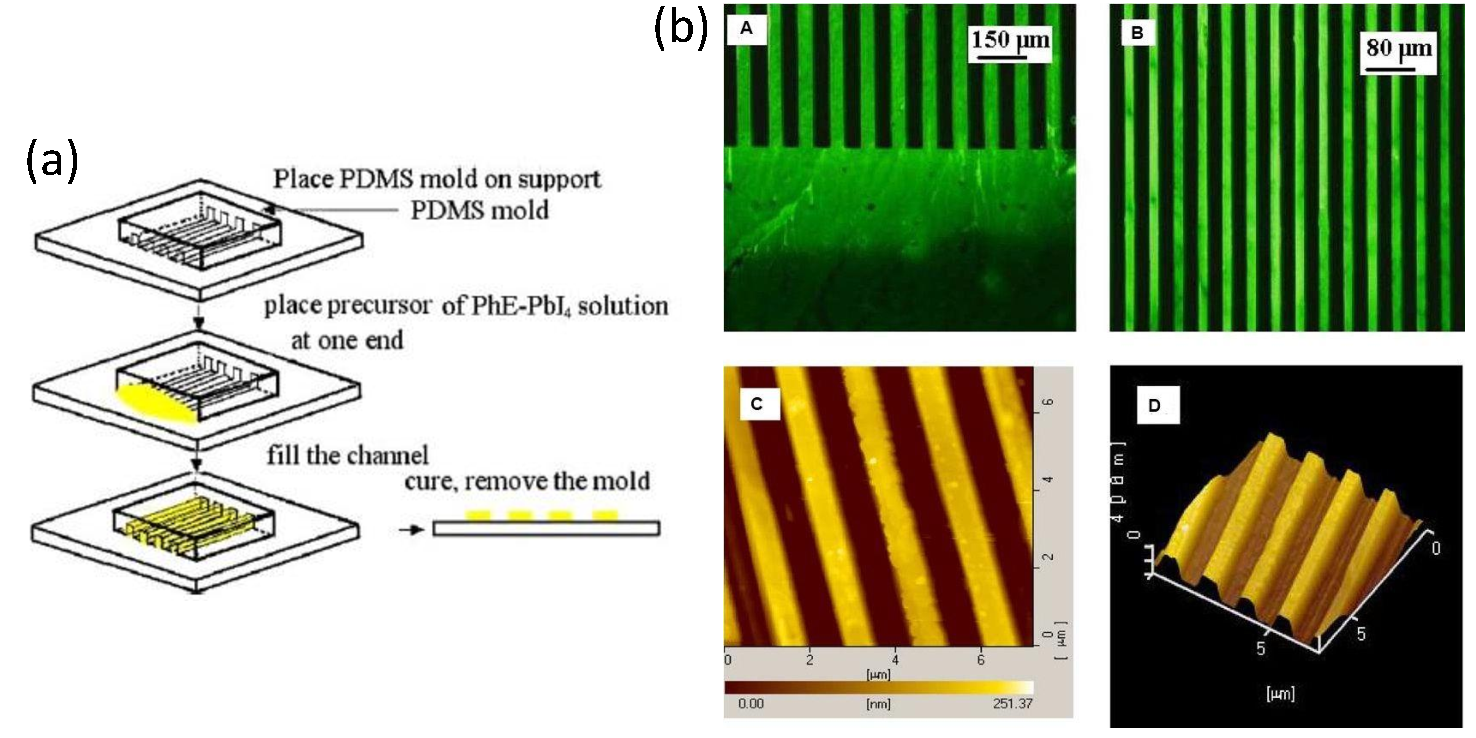
\includegraphics[width=\textwidth]{Fig11}
\caption{(a) Schematic of MIMIC process for pattering PAPI films. (b) Fluorescent optical micrographs (A,B) and AFM images (C: planar, D: stereo) of patterned PAPI films. In all cases the black stripes represent bare substrate without PAPI. Film stripe widths are A) 50\,$\mu$m wide, B) 15\,$\mu$m, C) and D) 0.8\,$\mu$m. Reproduced from Ref.\,\cite{Cheng2003}.}
\label{2Fig11}
\end{figure}


\subsection{Electronic structure}
\begin{figure}[h!]
\centering
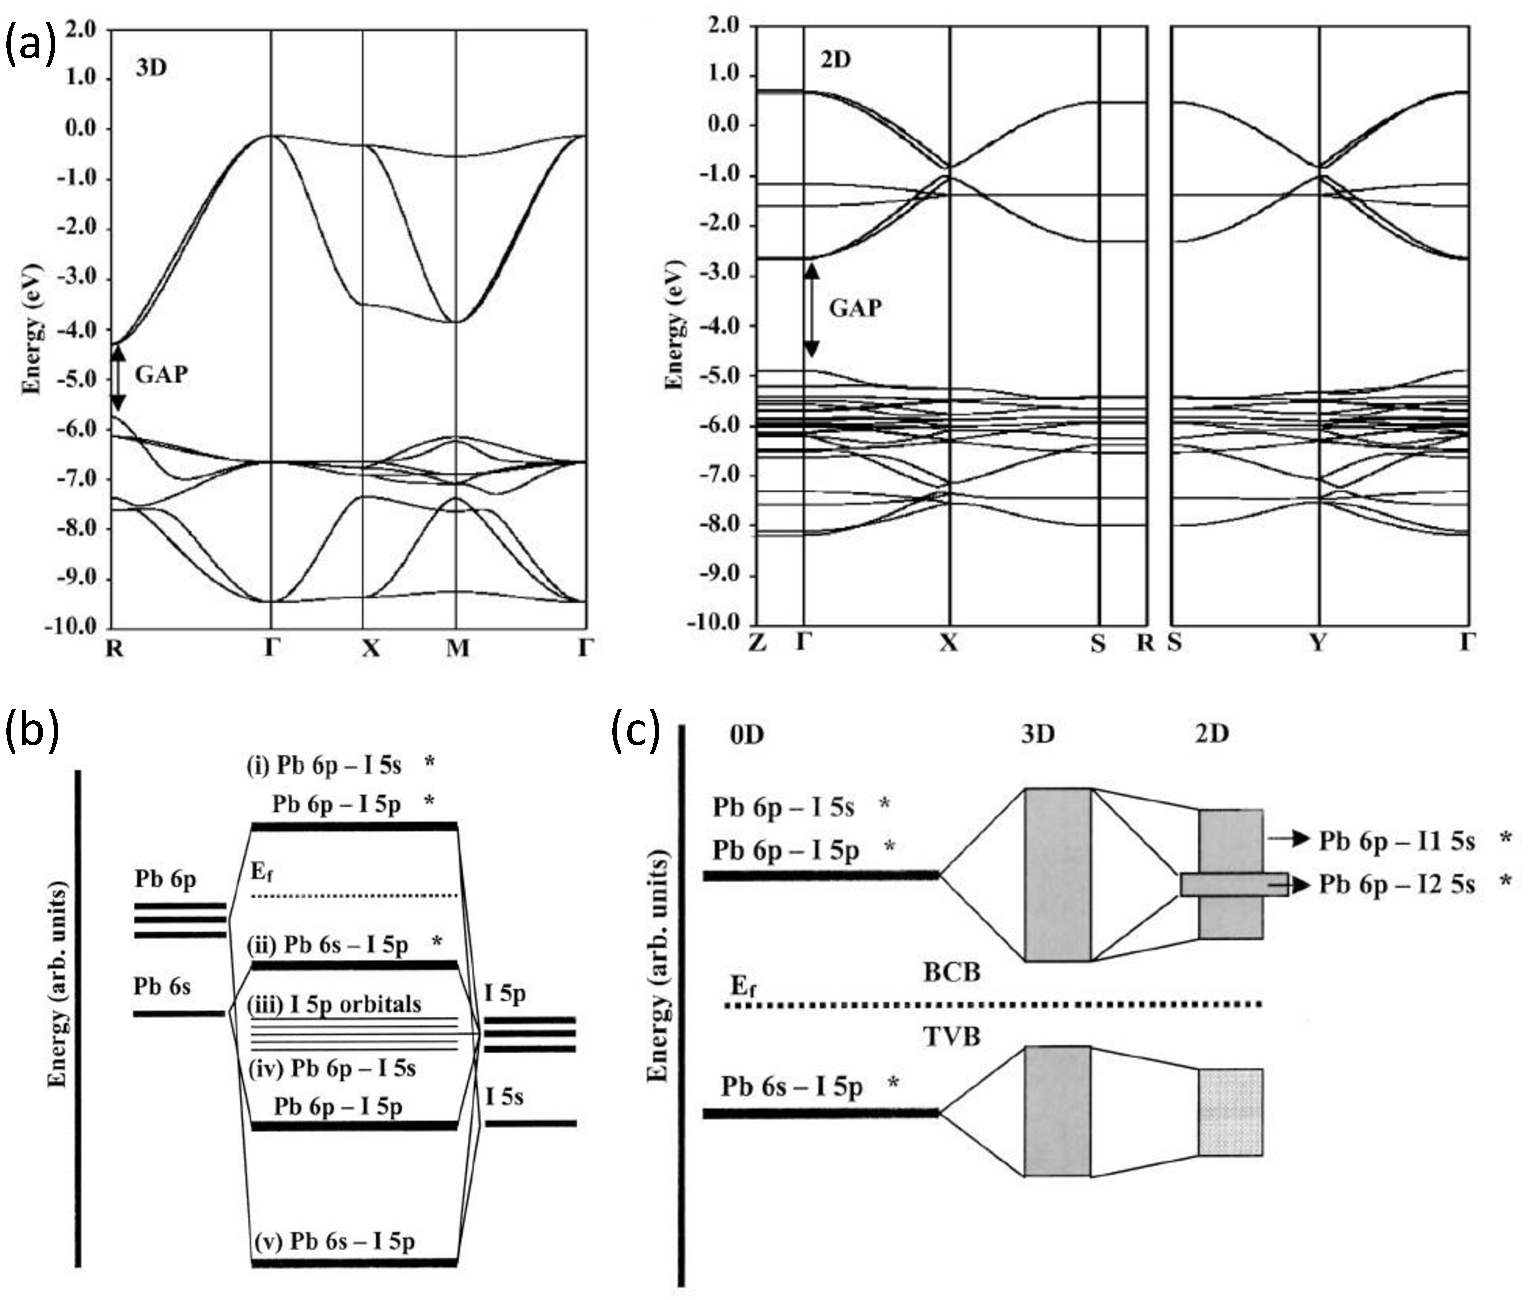
\includegraphics[width=\textwidth]{Fig12}
\caption{(a) Calculated band structures of $\textrm{CH}_3\textrm{NH}_3\textrm{PbI}_3$ (left) and $\textrm{C}_{4}$PI (right) along high symmetry lines in the first Brillouin zone. The band gap is labelled. Bonding diagrams of (b) one $\textrm{PbI}_6$ octahedron, and (c) extension to $\textrm{CH}_3\textrm{NH}_3\textrm{PbI}_3$ and $\textrm{C}_{4}$PI. The bottom of the conduction band (BCB), top of the valence band (TVB), and Fermi energy level ($\textrm{E}_F$) are labelled. Adapted from Ref.\ \cite{Umebayashi2003}.}
\label{2Fig12}
\end{figure}
Umebayashi \textit{et al.}\ calculated the electronic structure of $\textrm{C}_{4}$PI and its 3D extension $\textrm{CH}_3\textrm{NH}_3\textrm{PbI}_3$ using linear combination of atomic orbitals (LCAO) within density functional theory (DFT) [Fig.\,\ref{2Fig12}(a)] \cite{Umebayashi2003}. Both are direct gap semiconductors, but the 2D compound has a higher band gap and narrower bandwidths due to the decreased dimensionality. The 2D band structure also has flatter dispersions at the top of the valence band (TVB) and the bottom of the conduction band (BCB), leading to a larger carrier effective mass, and thus larger binding energy for excitons. 

Fig.\,\ref{2Fig12}(b) shows the bonding diagrams for a single $\textrm{PbI}_6$ octahedron, as well as the 3D and 2D compounds above. In the 2D crystal the TVB consists of Pb($6s$) and I($5p$) $\sigma$-antibonding orbitals, whereas the BCB consists of Pb($6p$) and I($5s$) $\sigma$-antibonding orbitals and Pb($6p$) and I($5p$) $\pi$-antibonding orbitals (not labelled on figure). The crystal field also lifts the degeneracy between different iodine atoms, so the conduction band with bridging iodine atoms ($\textrm{I}_1$) is wider than that with terminal iodine atoms ($\textrm{I}_2$). In Ref.\ \cite{Matsuishi2004} the BCB was labelled non-bonding from first principles pseudopotential total-energy calculations with the local density approximation, although it still consisted of Pb($6p$) and I($5p$) orbitals.

\subsection{Optical properties}
\subsubsection{Excitons}
\begin{figure}[h!]
\centering
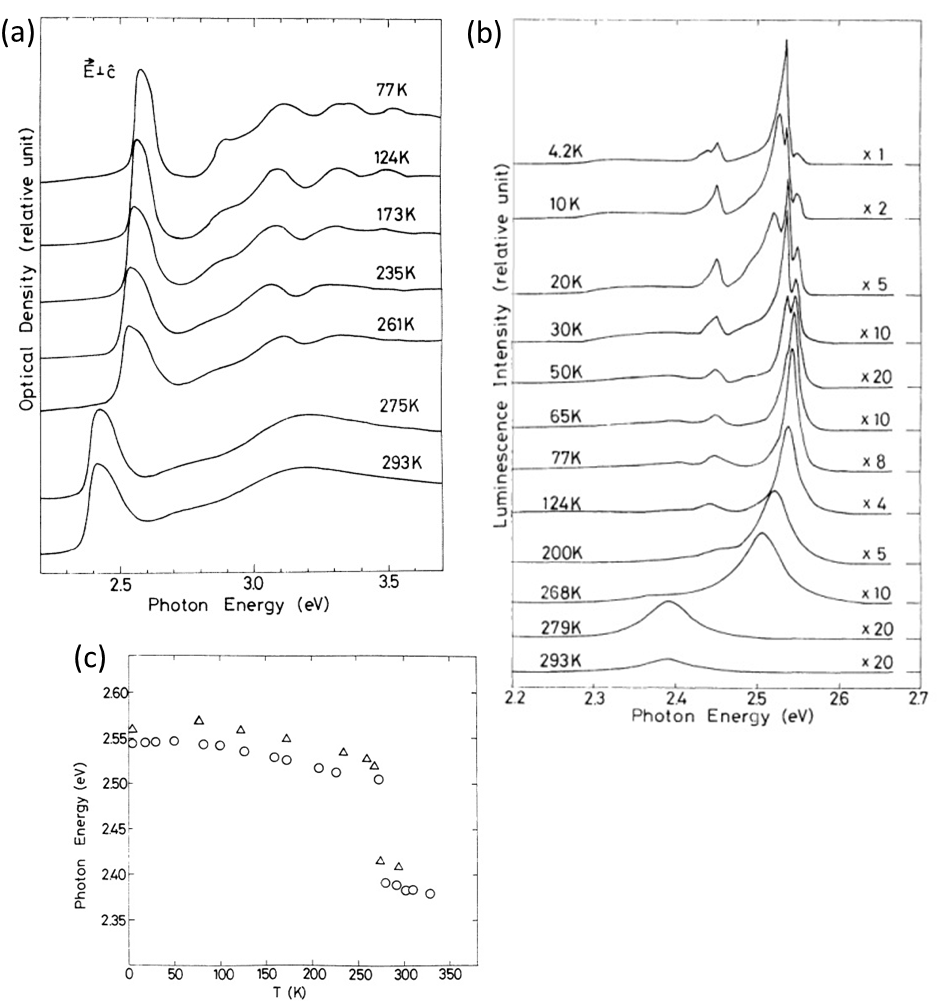
\includegraphics[width=\textwidth]{Fig13}
\caption{(a) Polarised optical density of $\textrm{C}_{10}$PI crystal at labelled temperatures, with $\vec{\mathbf{E}}$ parallel to the QWs. (b) Photoluminescence spectra spectra of $\textrm{C}_{10}$PI. The temperature and scaling of plotted data are labelled. (c) Energies of absorption ($\triangle$) and photoluminescence ($\circ$) peaks as a function of temperature. Reproduced from Ref.\ \cite{Ishihara1990}.}
\label{2Fig13}
\end{figure}
Excitons are formed due to transitions between the TVB and BCB in the inorganic layers of PbI perovskites. Excitons in $\textrm{C}_{10}$PI have an energy of 2.4\,eV above 275\,K, but the value changes to 2.55\,eV at below 268\,K due to a phase transition of the alkylammonium molecules [Fig.\ \ref{2Fig13}]. The binding energy $E_B$ is calculated from the difference between the exciton peak and the step-like structure (interband transitions) in absorption spectra, and the value of $320\pm10$\,meV explains the presence of excitons at room temperature. Excitons also have a large oscillator strength of around $0.7\pm0.1$ \cite{Ishihara1990}. The above values are for the lowest energy ($n=1$) free exciton, but bound excitons can also be seen, for example in Fig.\,\ref{2Fig13}(b) the peak at 2.55\,eV is assigned to the lowest free exciton in the inorganic layers, whereas the peak at 2.53\,eV decreases in intensity with temperature and is assigned to a shallowly bound exciton. The peaks seen at low temperature $\sim2.45$\,eV are sample dependent, and thus assigned to deeply impurity-bound excitons \cite{Ishihara1990}. The Stokes shift for $\textrm{C}_{10}$PI is less than 5\,meV [Fig.\,\ref{2Fig13}(c)], and this is generally true for PbI-based perovskites (e.g. for $\textrm{C}_{12}$PI in Ref.\,\cite{Pradeesh2009}). In Refs.\,\cite{Ishihara1990, Ishihara1989} both longitudinal and transverse exciton-polaritons are observed in reflection spectra of $\textrm{C}_{10}$PI at 1.6\,K, with a splitting of around 60\,meV \cite{Ishihara1990}. The exciton radiative lifetime is 7\,ps at 8\,K \cite{Kondo1998a}.

Polarisation-dependent excitons are seen in the Kramers-Kronig calculated absorption spectra of diammonium \ce{(H3NC6H13NH3)PbI} [Fig.\,\ref{2Fig14}]. When the incoming light is polarised parallel to the crystallographic $\vec{b}$ axis, the lowest exciton has an energy of 2.5272\,eV. Two shoulders seen at 2.566 and 2.718\,eV (indicated by small arrows) are due to vibronic bands. The very small peak at 2.819\,eV is attributed to $n=2$ excitons, as determined using exciton activation energies calculated from PL spectra. Due to the monoclinic crystal symmetry, light polarised parallel to $\vec{c}$ can generate excitons polarised along both the $\vec{a}$ and $\vec{c}$ axes. And as the $\vec{a}$ and $\vec{b}$ directions are very nearly isotropic, the peak at 2.5272\,eV (also seen in Fig.\,\ref{2Fig14}(a)), is attributed to excitons polarised parallel to $\vec{a}$. The narrow peak at 2.559\,eV is due to excitons polarised parallel to $\vec{c}$, but only appears at very low temperatures as the linewidth normally causes the two exciton peaks to be indistinguishable. The binding energy for the material is calculated to be 330\,meV, and the Bohr radius 8.2\,\AA \cite{Goto2001}.
\begin{figure} [h!]
\centering
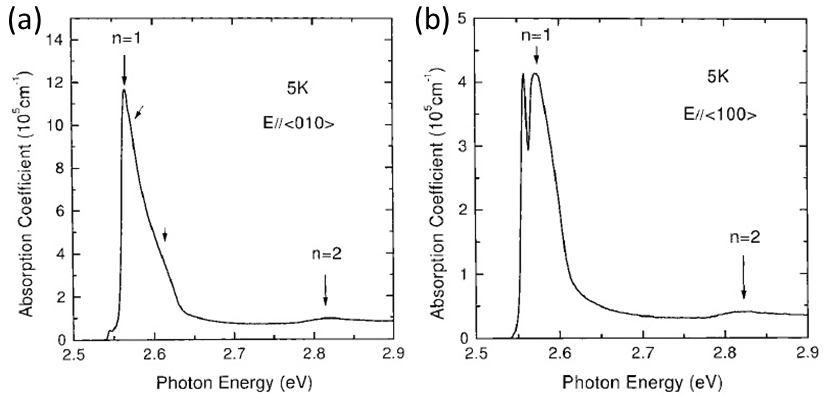
\includegraphics[width=\textwidth]{Fig14}
\caption{Absorbance spectra for $\vec{\mathbf{E}}$ parallel to (a) $\vec{b}$, and (b) $\vec{c}$ axes for \ce{(H3NC6H13NH3)PbI4}, calculated using Kramers-Kronig relations from reflection spectra. The $n=1, 2$ peaks are labelled, and arrows indicate vibronic sidebands. Reproduced from Ref.\ \cite{Goto2001}.}
\label{2Fig14}
\end{figure}

The band gap of perovskites can be engineered by altering the halogen and metal atoms in the structure. The exciton energy ranges from 2.5\,eV for PbI perovskites, to 3.1\,eV for PbBr and 3.6\,eV for PbCl. Indeed mixed-halide perovskites of the form \ce{(RNH3)2Pb}$\textnormal{A}_x\textnormal{B}_{1-x}$ allow variation within this range \cite{Kitazawa1996, Kitazawa1997}. It has been shown that the while the change in absorption wavelength generally varies linearly with the halogen concentration $x$, because the process is averaged over excitons at all possible sites, the excitons formed then preferentially diffuse over $\sim10$\,nm to lower energy halogen atomic sites so the emission wavelength does not show the same linear variation with $x$ \cite{Ahmad2013}.

There has been some discussion regarding the nature of the excitons. Xu \textit{et al.} used magneto-optical measurements on polycrystalline $\textrm{C}_{10}$PI thin films and found that exciton peaks are not shifted when a magnetic field is applied in the plane of the QWs. However when the field is perpendicular to the QWs the energy of the exciton $E$ changes according to
\begin{equation}
E = E_0 \pm \frac{1}{2} g_{\bot} \mu_{B} B + c_0 B^2~,
\label{mag-shift}
\end{equation} 
where $E_0$ is the energy of the exciton at zero field, $g_{\bot}$ is the Land\'{e} $g$ factor perpendicular to the plane of the film, $\mu_B$ is the Bohr magneton, and $c_0$ is the diamagnetic constant. The sign of the energy shift depends on the polarisation of the magnetic field, and from the data $g_{\bot}\sim1$, and $c_0\sim 10^{-7}$~eV/$\textrm{T}^2$ for C$_{10}$PI. From the magneto-absorption measurements $a_B \sim12\,$\AA for $\textrm{C}_{10}$PI. The peak shifts indicate $\textrm{C}_{10}$PI excitons are Wannier-like, since Frenkel excitons would have no extended motion and thus show no energy shift at all. However as the size of each $\textrm{PbI}_6$ octahedron is around 6\,\AA~\cite{Ishihara1990}, excitonic motion extends over only a few octahedra \cite{Xu1991b}.

Magneto-optical measurements on C$_6$PI produces $g_{\bot}$ and $c_0$ values similar to those in $\textrm{C}_{10}$PI, however the authors believed that as the exciton Bohr radius is on the order of Pb-Pb distances in the crystal, the exciton may be better described by a cationic Frenkel model involving orbitals of Pb$^{2+}$. The calculated $g_{\bot}$ and $c_0$ agree well with experiment \cite{Kataoka1993}. On the other hand Tanaka \textit{et al.}\ used electroabsorption and two-photon absorption studies and showed that excitons in thin film $\textrm{C}_{6}$PI samples were Wannier-like in nature, with 1s, 2s, 2p, and 3p energies at 2.34, 2.60, 2.61, and 2.64\,eV respectively. The Wannier excitons exhibited strong 2D behaviour, and for the 1s exciton $E_B = 310$\,meV \cite{Tanaka2002}.


\subsubsection{Biexcitons and triexcitons}
\begin{figure}[h!]
\centering
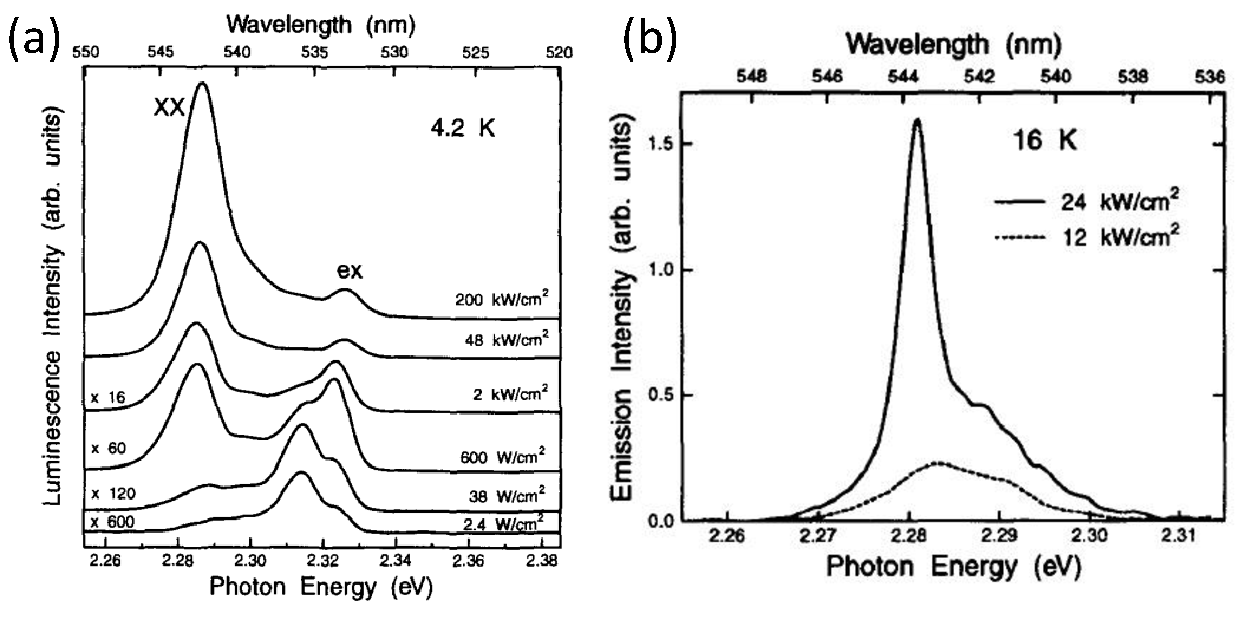
\includegraphics[width=\textwidth]{Fig15}
\caption{(a) Photoluminescence spectra of $\textrm{C}_{6}$PI film excited by 337\,nm nitrogen laser at 4.2\,K. The excitation intensity and data scaling are given. Exciton (ex) and biexciton (XX) bands are labelled. (b) Emission spectra of $\textrm{C}_{6}$PI waveguide above (24\,kW/$\textrm{cm}^2$) and below (12\,kW/$\textrm{cm}^2$) the lasing threshold at 4.2\,K. The lasing wavelength is 543.6\,nm. Reproduced from Ref.\,\cite{Kondo1998}.}
\label{2Fig15}
\end{figure}
An increase in excitation power can lead to the formation of bi- or tri-exciton complexes, where two or three free excitons are bound together. Induced photo-carriers screen Coulomb interactions, so strong interactions between carriers are needed to observe triexcitons. Low dimensionality is an advantage as screening has a more limited effect \cite{Shimizu2006a}. The radiative decay of biexcitons to transverse excitons has been observed in \ce{C6PI} [Fig.\,\ref{2Fig15}(a)] and $\textrm{C}_{10}$PI, with biexciton binding energy of $\sim50$\,meV \cite{Kondo1998, Ishihara1992}. By creating a waveguide configuration with transverse pumping, biexciton lasing is observed in $\textrm{C}_6$PI. The lasing threshold is 20\,kW/$\textrm{cm}^2$ at 16\,K. Fig.\ref{2Fig15}(b) shows emission spectra above and below the lasing threshold: a broad biexciton band is seen below the threshold, but a sharp peak at 2.281V can be observed above the threshold. The biexciton band is probably isotropic as the emission is not polarised \cite{Kondo1998}.

\begin{figure}[h!]
\centering
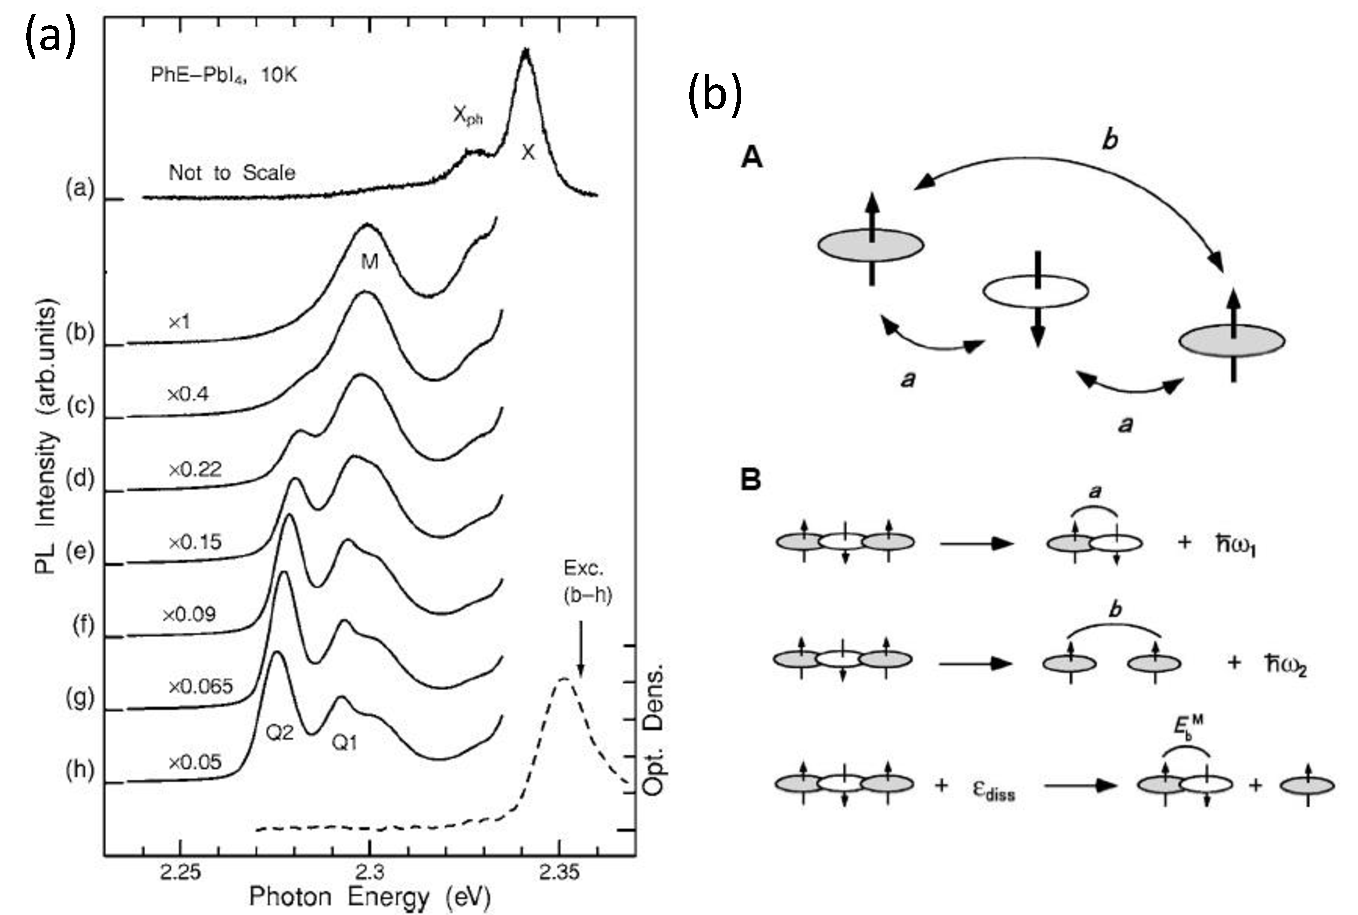
\includegraphics[width=\textwidth]{Fig16}
\caption{(a) PL spectra of PAPI at different excitation intensities and energies. (a) is excited at 2.58eV, and (b)-(h) at 2.355eV. The excitation intensities are (a) $4.6\times 10^{10}$, (b) $4.6\times 10^{12}$, (c) $1.4\times 10^{13}$, (d) $2.8\times 10^{13}$, (e) $4.6\times 10^{13}$, (f) $9.2\times 10^{13}$, (g) $1.6\times 10^{14}$, and (h) $3.2\times 10^{14}$ photons c$\textrm{m}^{-2}$. The dotted line shows the absorption spectrum. X is the free exciton band, $\textrm{X}_{\textrm{\footnotesize ph}}$ phonon sidebands, M the biexciton band, $\textrm{Q}_1$ amplified spontaneous recombination of biexcitons, and $\textrm{Q}_2$ the $\hbar \omega_2$ triexciton process. (b) A) shows the triexciton model, and B) likely dissociation mechanisms. For the meaning of symbols see the main text. Reproduced from Ref.\cite{Shimizu2006a}.}
\label{2Fig16}
\end{figure}

Shimizu \textit{et al.}\ observed triexciton formation in the PL spectra of PAPI. In Fig.\ \ref{2Fig16}(a), the free exciton band is labelled X, phonon sidebands $\textrm{X}_{\textrm{\footnotesize ph}}$, and the biexciton band M. At higher excitation intensities, two other bands can be seen, labelled $\textrm{Q}_1$ and $\textrm{Q}_2$. $\textrm{Q}_1$ is assigned to the amplified spontaneous emission due biexciton recombination, and $\textrm{Q}_2$ to a triexciton process. Triexcitons consist of bound states of three spin singlet excitons, with interaction energy $a$ between opposite spin excitons ($<0$), and interaction energy $b$ between same spin excitons ($>0$). Likely radiative triexciton dissociation mechanisms are dissociation into a biexciton and photon $\omega_1$, or two excitons and photon $\omega_2$. However nonradiative dissociation (energy $\epsilon_{\textrm{\footnotesize diss}}$) into a biexciton (binding energy $E_{\textrm{\footnotesize b}}^{\textrm{\footnotesize M}}$) and an exciton is also possible [Fig.\,\ref{2Fig16}(b)]. As $\textrm{Q}_2$ is at a lower energy than M, it can only be due to the $\omega_2$ process, although it is unclear why the $\omega_1$ process is not observed. From the data collected, $a=-37.5$\,meV, $b=11$\,meV, $\epsilon_{\textrm{\footnotesize diss}}=14$\,meV, and $E_{\textrm{\footnotesize b}}^{\textrm{\footnotesize M}}=50$\,meV \cite{Shimizu2006a}. 


\subsubsection{Dielectric confinement and the image charge effect}

Both the binding energy and oscillator strength of (transverse) excitons in 2D PbI perovskites are much larger than those in the inorganic 3D equivalent Pb$\textrm{I}_2$ \cite{Hirasawa1994}. In materials where a QW is sandwiched between barrier layers with lower dielectric constant $\epsilon_b$, three types of confinement affect excitons. Firstly quantum confinement, where the reduction in dimensionality to 2D gives a binding energy four times larger than expected in bulk 3D material for the $n=1$ exciton as discussed in Section \ref{sec:ex2D} \cite{Shinada1966}. Secondly dielectric confinement, where the lower barrier $\epsilon_b$ reduces the effective dielectric constant of the entire structure, thus providing less shielding and giving a higher binding energy. Thirdly mass confinement, where carrier wavefunctions extending into the barrier region lead to a larger effective mass, thus increasing the binding energy. Mass confinement depends on quantum confinement in order to determine how much of the carrier wavefunction is leaked into the barrier region, and generally only has a small effect \cite{Kumagai1989}. The interfaces between layers also act as mirrors which create an infinite series of image charges [Fig.\ \ref{2Fig17}]. Using carrier wavefunctions which fit the boundary conditions of the well, as well as self and image-charge Hamiltonians, exciton properties can be calculated. The results show that $E_B$ increases if the barrier height decreases, the excitons have larger effective mass in carrier region, or the barrier regions have a smaller dielectric constant \cite{Kumagai1989}. Muljarov \textit{et al.}\ found that the potentials created due to the image charge effect causes charges in the inorganic layers to be repelled from the interface, whereas charges in the organic layers are attracted to the interface \cite{Muljarov1995}.
\begin{figure}[h!]
\centering
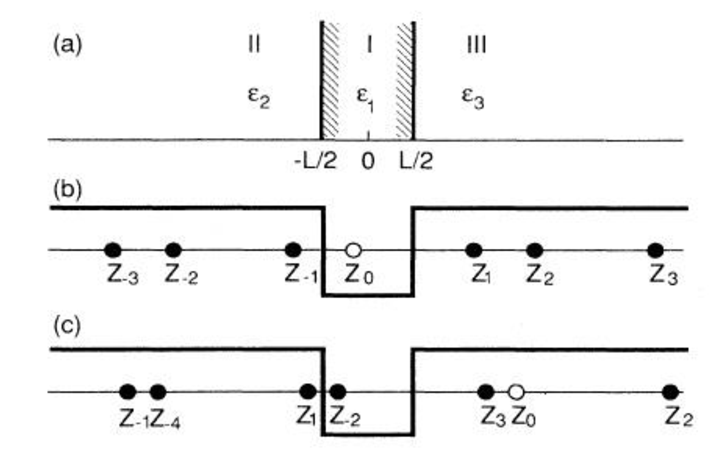
\includegraphics[width=0.8\textwidth]{Fig17}
\caption{(a) Generalised description of quantum well (region I) and barriers (regions II and III). (b) and (c) show the positions of initial charges (white circle, $Z_0$) and image charges created (black circles) due to interfaces. In (b) the initial charge is in the well region, whereas in (c) it is in the barrier region. Reproduced from Ref.\ \cite{Kumagai1989}.}
\label{2Fig17}
\end{figure}

\subsection{Organic molecules}
The way organic molecules fit into the perovskite structure can change the conformation of \ce{PbI6} octahedra, the Pb-I bond angle or the interlayer I-I coupling, all of which lead to a change in the electronic structure \cite{Sourisseau2007}. Pb-I-Pb bond angles have the greatest effect on the band gap of perovskites. Experimental results show that bond angles closer to $180^{\circ}$ (undistorted octahedra) lead to smaller $E_g$, which agrees with extended Huckel tight-binding calculations used to evaluate band structures of PbI perovskites [Fig.\ \ref{2Fig19}]. Although $E_g$ is underestimated using this model, the overall correlation between I-Pb-I angle and electronic energy levels are correct \cite{Pradeesh2009}. Calculations for Sn-based perovskites show that bond angle distortions in the QW plane have a larger impact on $E_g$ than purely out-of-plane distortions \cite{Knutson2005}. For this reason, pressure can be used as an external parameter to tune to exciton energy \cite{Matsuishi2001}.
\begin{figure}[h!]
\centering
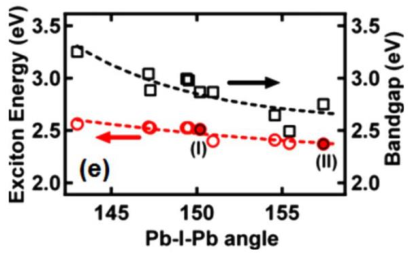
\includegraphics[width=0.6\textwidth]{Fig19}
\caption{Variations in exciton energy (red) and band gap (black) with Pb-I-Pb angles calculated using extended Huckel tight binding calculations. Data points given are experimentally determined for PbI perovskites, and filled in circles represent PL maxima of labelled $\textrm{C}_{12}$PI phases. Reproduced from Ref.\ \cite{Pradeesh2009}.}
\label{2Fig19}
\end{figure}

2,$2^{'}$-biimidazole ($\textrm{C}_6\textrm{H}_6\textrm{N}_4$) can be incorporated into the perovskite structure to form $(\textrm{C}_6\textrm{H}_8\textrm{N}_4)\textrm{PbI}_4$. The loss of \ce{NH3} groups, as well as the ability to delocalise charge across the organic molecule, leads to weaker hydrogen bonding with inorganic octahedra. Thus the reduced corrugation of QWs produces smaller $E_g$ compared to C$_n$PI \cite{Tang2001}. Similarly in $(\textrm{HO(CH}_2)_2\textrm{NH}_3)_2\textrm{PbI}_4$, the OH group is able to hydrogen bond with neighbouring $\textrm{NH}_3$ groups or I atoms. The extra interactions weaken the $\textrm{NH}_3$-I hydrogen bonds, and also provide a channel for stronger electronic coupling between inorganic layers, leading to smaller $E_g$ \cite{Mercier2004}.

In general perovskites have better PL efficiencies if the QWs are flat. Therefore as well as bonding with functional groups of the organic molecule, the most emissive compounds are created using relatively flexible molecules whose size allows the formation of the MQW structure without too much deformation of inorganic sheets \cite{Zhang2009}.

As well as structural effects, notable properties of the organic ligand can be be incorporated into the perovskite. For example perovskites with with chiral molecules also exhibit optical activity \cite{Teshima2003}, while inclusion of chromophores into the structure can lead to charge and energy transfer between the organic and inorganic layers \cite{Kawabata2009, Mitzi1999a, Braun1999}.

\subsection{Applications}
\subsubsection{Microcavities and photonic crystals}
The dynamics of interactions between quasiparticles can be described in two limiting regimes. In the weak coupling limit the system can still be described by the original quasiparticle wavefunctions, albeit with some perturbations. In the strong coupling limit, coherent interactions between quasiparticles lead to the formation of mixed states that oscillate between the original eigenstates with frequency $\Omega_R$ (Rabi frequency, also a measure of the interaction strength). The new mixed states can combine properties of both the original particles. For example, strong coupling between excitons and cavity photon modes create exciton-polaritons, quasiparticles with small effective mass but capable of nonlinear interactions, polaritons have shown great promise in producing Bose-Einstein condensates \cite{Kasprzak2006}, low-threshold lasers \cite{Christopoulos2007} and ultrafast switches \cite{Amo2010}.
\begin{figure}[h!]
\centering
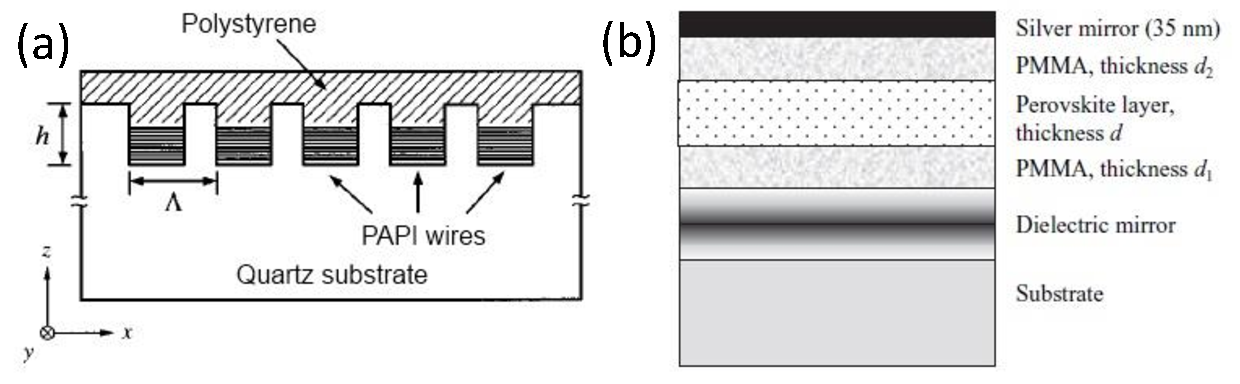
\includegraphics[width=\textwidth]{Fig20}
\caption{(a) Schematic of a distributed feedback microcavity. (b) Transmission dip positions at normal incidence as a function of cavity detuning from the PAPI exciton energy. Closed circles and diamonds represent the upper and lower polariton branches respectively, while closed squares indicate upper branch polaritons not affected by the reciprocal lattice vectors. Reproduced from Ref.\ \cite{Fujita1998}.}
\label{2Fig20}
\end{figure}

Strong coupling has been observed between PAPI excitons and cavity modes in a distributed feedback microcavity at room temperature \cite{Fujita1998, Fujita1999, Fujita2000}. The cavity consists of a structured quartz substrate with PAPI spin coated into the spaces to form parallel wires, and an overcoat of polystyrene added to prevent the degradation of PAPI films [Fig.\,\ref{2Fig20}(a)]. When the incident beam is at normal incidence, PAPI excitons and fourth order cavity resonance become resonant, couple strongly and form new eigenstates (cavity polaritons). Using a variety of grating pitches $\Gamma$ from 0.62 to 0.72\,$\mu$m, transmission spectra showed that the upper and lower polariton branches exhibit anticrossing behaviour, as expected for strongly coupled modes [Fig.\,\ref{2Fig20}(b)]. Due to the large exciton oscillator strength, the mode splitting is around 100\,meV, an order of magnitude larger than the 9\,meV observed in GaAs systems in Fabry-Perot microcavities \cite{Fujita1998}. A strong enhancement of PL intensity of the lower branch polariton is seen if the standing wave cavity mode is in resonance with PAPI excitons, in this case when $\Gamma=0.68\,\mu$m \cite{Fujita1999}. No signature of the upper polariton branch is seen as in thermodynamic equilibrium the upper branch would expect to be less populated, however the polariton lifetime may not be long enough for equilibrium to occur. Other suggestions have included a relaxation of the upper branch polaritons towards uncoupled excitonic states, or fast emission of photons between the upper and lower polariton branches \cite{Lanty2008}. It is thought that PAPI rods oscillating in phase due to strong coupling with cavity modes at resonance would lead to a macroscopic polarisation and ultrafast resonance, however the polariton lifetime is actually 8\,ps longer with a grating structure at 40\,K. It is possible that this is due to excitons with large wave vectors that cannot couple to the outside without the help of the grating reciprocal lattice vector \cite{Fujita2000}. Strong coupling between excitons and 2D grating modes has also been observed in PAPI with Rabi splitting 100\,meV \cite{Ishi-Hayase2003}.

Strong coupling between cavity and PAPI exciton modes are also observed in the Fabry-Perot microcavities \cite{Brehier2006, Lanty2008}. By adjusting the position of the perovskite layer in the microcavity, the coupling between exciton and photon modes can be controlled, and the splittings seen were between 130-190\,nm. Similar CHPI microcavities constructed produce splittings of 130\,meV for a $5\lambda/4$ metal-air microcavity, and of 160\,meV for a $7\lambda/4$ metal-metal microcavity \cite{Pradeesh2009b}.

Strong exciton-photon coupling has also been observed in a photonic crystal of 256\,nm diameter microspheres infiltrated with PAPI (silica opal) \cite{Sumioka2001}. A face centred cubic lattice of silica microspheres with 3D channel voids is created, and a solution of PAPI and DMF introduced into continuous spaces through capillary forces [Fig.\,\ref{2Fig21}(a)]. Angle-dependent reflectivity spectra of the structure with PAPI filling fraction $f_{\textnormal{PAPI}}=0.06$ clearly demonstrates anticrossing behaviour, indicating strong coupling between the stop band (photon mode) of the photonic crystal and the exciton mode of PAPI, with Rabi splitting 240\,meV [Fig.\,\ref{2Fig21}(b)]. However there is an uncoupled exciton mode that seems largely unaffected by the photon mode, possibly due to some of the bulk PAPI on the surface of the silica opal remaining, or an open photonic gap in the silica opal that leads to insufficient photon confinement and limits exciton-photon coupling. 
\begin{figure}[h!]
\centering
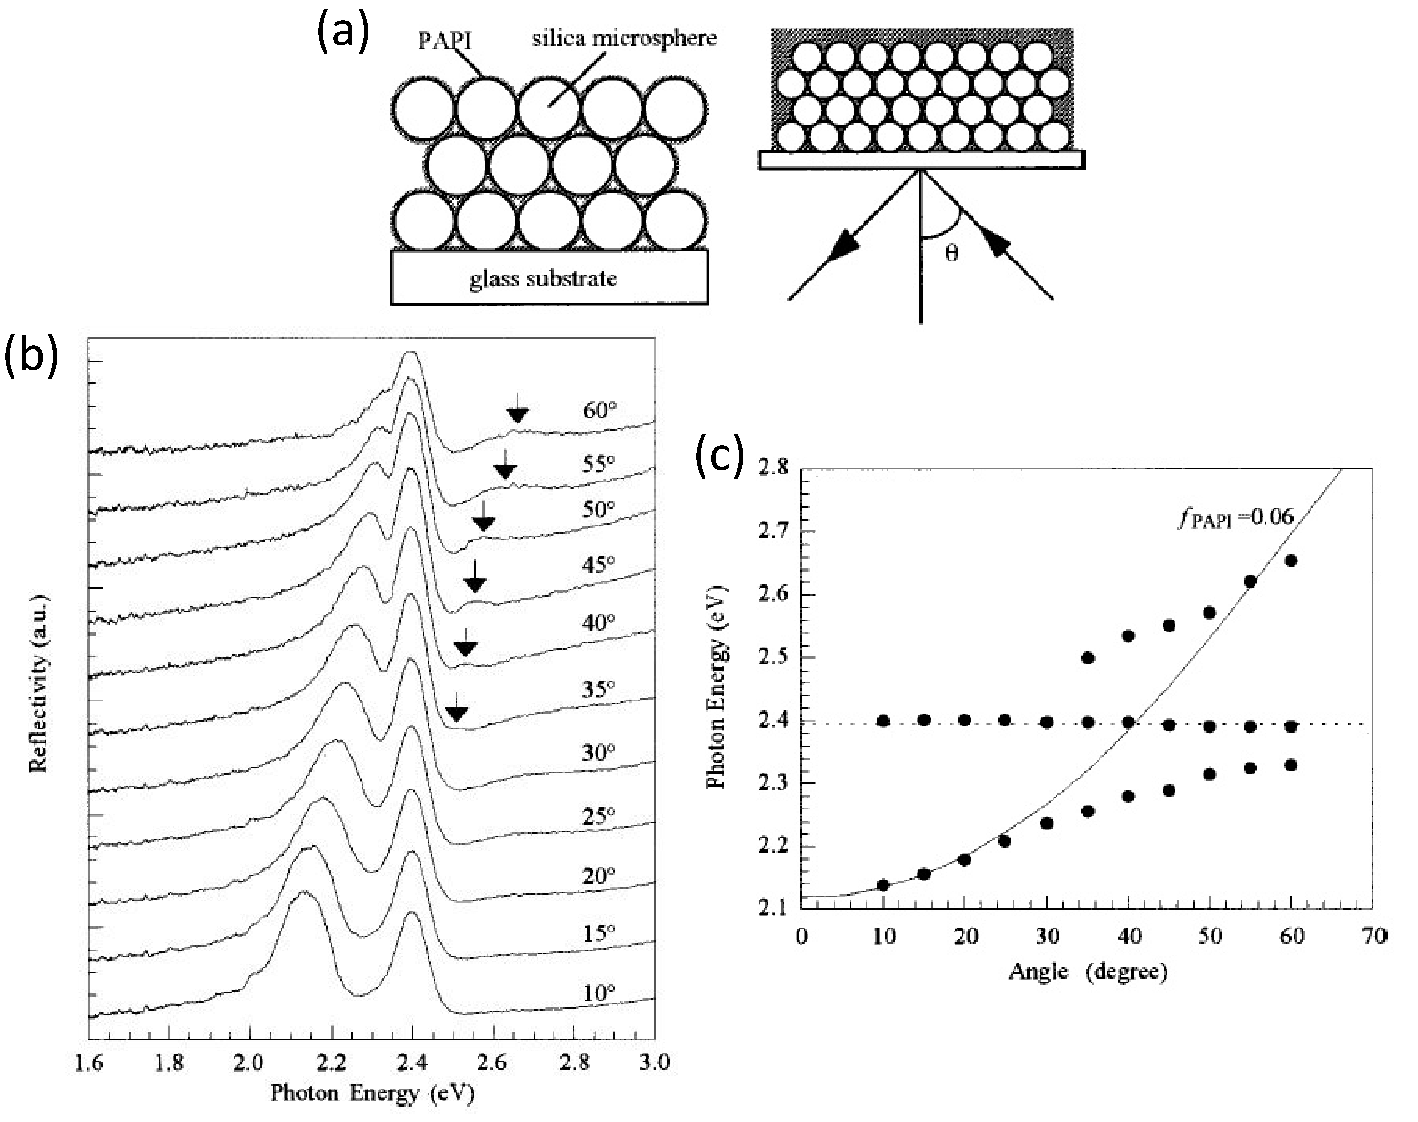
\includegraphics[width=\textwidth]{Fig21}
\caption{(a) Structure of silica opal infiltrated with PAPI film formed on a glass substrate. (b) Extracted mode positions from angle-dependent reflectivity spectra (black circles) for opal with PAPI filling fraction $f_{\textnormal{PAPI}}=0.06$. Exciton energy (dashed line) and theoretical photonic crystal stop gap (solid line) are marked. Reproduced from Ref.\ \cite{Sumioka2001}.}
\label{2Fig21}
\end{figure}

\subsubsection{Optoelectronic devices}
The processability of perovskites from solution and their high PL efficiencies make perovskites attractive for optoelectronic devices, particularly electroluminescent (EL) devices. Era \textit{et al.}\ used a layered structure consisting of PAPI, an indium-tin-oxide (ITO) anode, MgAg cathode, and oxadiazole (OXD7) electron transport layer [Fig.\,\ref{2Fig22}(a)]. When the device is driven, electrons in OXD7 are injected smoothly into the PAPI layer as there is no energy barrier, but holes injected into PAPI will remain at the PAPI/OXD7 interface due to the barrier potential [Fig.\,\ref{2Fig22}(b)]. Electrons and holes are therefore trapped in the PAPI layer, and recombine to provide luminescence. When driven at liquid nitrogen temperatures, the EL intensity reaches a luminescence of more than 10000\,cd$\textrm{m}^2$ at a current density of 2\,A$\textrm{cm}^{-2}$ and voltage of 24\,V. The emission peak at 520\,nm has narrow bandwidth, and is very similar to the PL spectrum. However the EL efficiency at room temperature is much smaller than that at liquid nitrogen temperatures, and is mainly caused by thermal ionisation of excitons \cite{Era1994}. Similar devices made by Matsushima \textit{et al.} [Fig.\,\ref{2Fig22}(c)] show that an additional buffer layer (OTS=octadecyltrichlorosilane, CuPc=Cu pthalocyanine) can reduce the hole-injection barrier between ITO and PAPI, leading to an increase in EL efficiency. Buffer layers that decrease PAPI film roughness will also reduce leakage current \cite{Matsushima2005}.
\begin{figure}[h!]
\centering
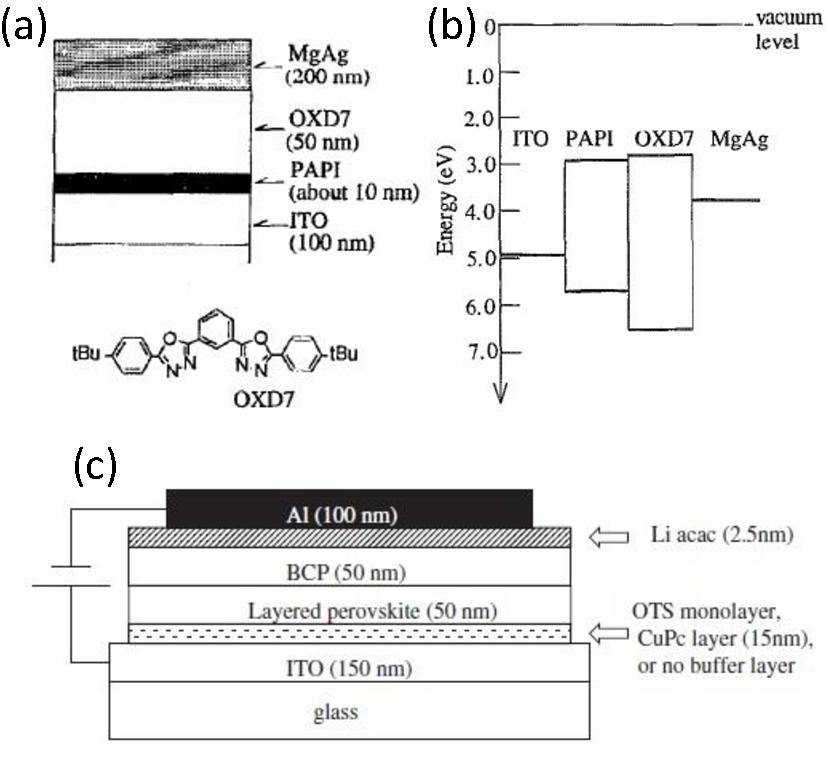
\includegraphics[width=0.8\textwidth]{Fig22}
\caption{(a) Schematic of EL device with PAPI by Era \textit{et al.}, and (b) energy level diagram of the device. (c) Schematic of the LED made using PAPI by Matsushima \textit{et al.}. (a-b) reproduced from Ref.\cite{Era1994}, (c) from \cite{Matsushima2005}.}
\label{2Fig22}
\end{figure}

Hattori \textit{et al.}\ made EL devices shown in Fig.\,\ref{2Fig22}(a) using PAPI, PBPI (\ce{(C6H5C4H8NH3)2PbI4}) and CHPI. As before the EL and PL of all three compounds are almost identical [Fig.\,\ref{2Fig23}(a)], however despite PBPI and CHPI having higher PL efficiencies than PAPI [Fig.\,\ref{2Fig23}(b)], the PBPI device had the lowest external quantum efficiency $\eta_{ext}$ (number of emitted photons/number of electrons) and CHPI the highest. The PBPI device is also much more resistive than the others, with current density around two orders of magnitude less than other devices at same voltage. Both the resistance and the low EL efficiency are likely due to the longer alkyl chain preventing carrier transport. The external efficiency of the CHPI device is comparable to the highest efficiency reported in EL devices reported at the time \cite{Hattori1996}.
\begin{figure}[h!]
\centering
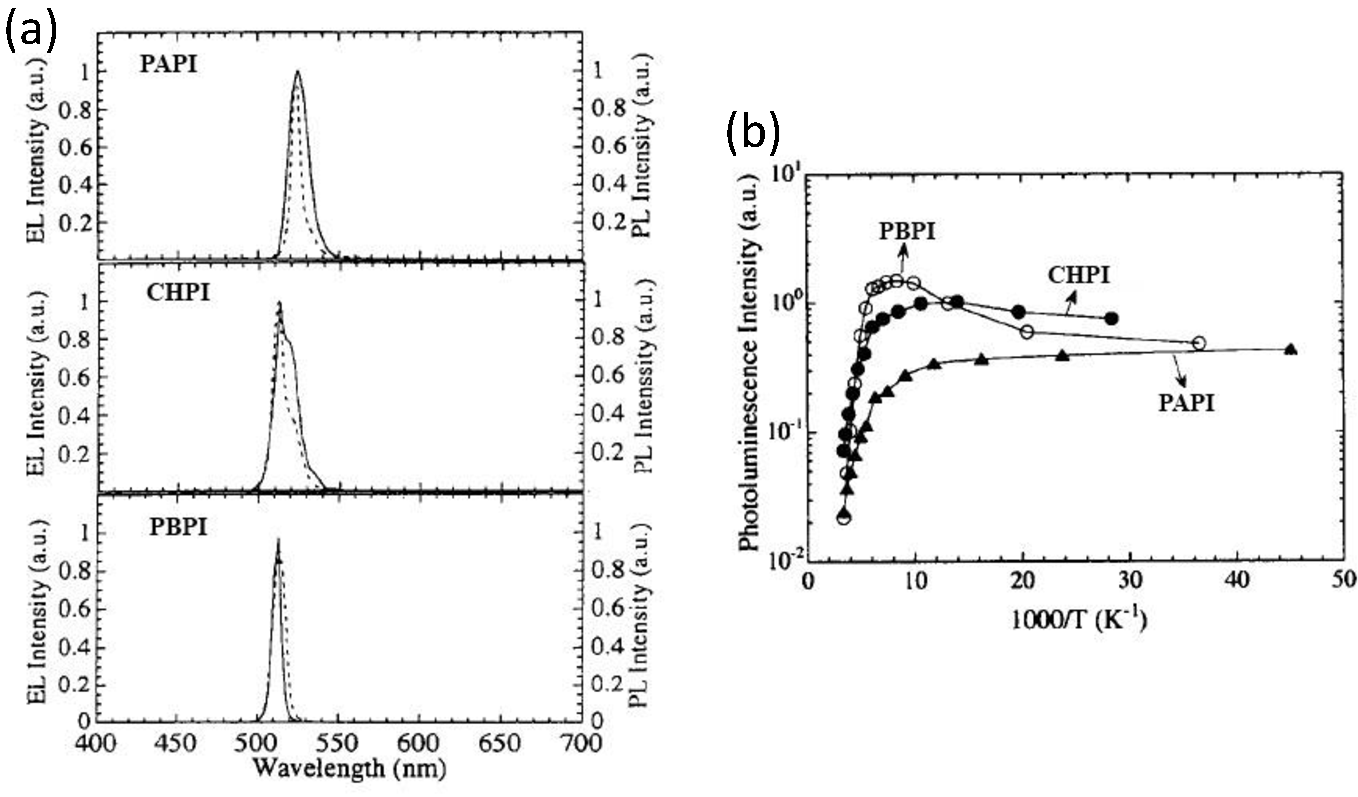
\includegraphics[width=0.6\textwidth]{Fig23}
\caption{(a) EL (solid lines) and PL (dotted lines) spectra of the labelled perovskite at 110\,K. EL device structure is shown in Fig.\ \ref{2Fig22}(a). (b) Integrated PL intensity of CHPI, PAPI, and PBPI thin film samples as a function of temperature. Reproduced from Ref.\ \cite{Hattori1996}.}
\label{2Fig23}
\end{figure}

Although there have not been many studies on the transport properties of 2D PbI perovskites, SnI perovskites have received more attention in this area. 2D SnI structures are semiconducting, while the 3D SnI perovskite is a low-carrier density p-type metal \cite{Mitzi1994}. Thin film transistors have also been produced from 2D SnI perovskites, with carrier mobilities of up to 1.4\,cm$^2$/Vs, better than that of amorphous silicon, with on-off ratio $>1000$ and current densities $>400$\,A/cm$^2$ \cite{Mitzi2002b, Mitzi2001d, Kagan1999a}.

\subsubsection{Scintillators}
Scintillators convert radiation energy into photo-emission for the purpose of detecting ionising radiation. They need to have a short luminescence decay time constant in order to react quickly, high resistance to radiation damage, and high efficiency so that a suitable number of photons are created per unit radiation energy of absorbed \cite{Shibuya2002}. Many efficient scintillators (e.g.\ NaI:TI, CsI:Na) have decay times of 200\,ns or more, whereas fast scintillators (e.g.\ Ba$\textrm{F}_2$, CsF) have low light yields of less than 2000~photons per MeV \cite{Kengo2002}. $\textrm{C}_6$PI crystals are bombarded by an ultra-short electron beam with pulse width of 1-2\,ps, generated by a 35MeV linear accelerator, and produced a decay constant of 45\,ps at room temperature \cite{Kengo2002}. Investigations show 2D perovskites have faster decay times than their 3D counterparts as quantum confinement provides carrier wavefunction overlap and higher likelihood of decay.

Shibuya \textit{et al.}\ used different dosages of 2\,MeV protons to test $\approx250$nm thick $\textrm{C}_6$PI thin films \cite{Shibuya2002}. Radiation-induced emission spectra show no shift in the exciton peak position during bombardment, and no additional peaks appeared at any radiation dosage. Three decay components are found: one with decay constant 0.39\,ns due to free exciton recombination, then two defect density dependent components with constants of 3.8 and 16\,ns due to trapped excitons, with decay constants depending on defect density. Emission intensities of $\textrm{C}_6$PI excitons attenuated with increased radiation, but the radiation hardness is still enough for practical use. From these results, $\textrm{C}_6$PI is a good candidate for scintillator use due to the stability of excitons at room temperature, ease of processing, fast response time, spectrum stability to radiation, and inclusion of high atomic number element (Pb) in order to detect low energy transfer radiation such as X-rays \cite{Shibuya2004}. 

\section{Conclusions}
Excitons, bound hydrogen atom-like systems of electrons and holes, produce strong optical signatures in semiconductors, and many exciton effects are enhanced by a reduction in dimensionality. 2D hybrid organic-inorganic perovskites are naturally self-assembling materials that create a MQW structure, whose room temperature optical properties are dominated by the excitons produced in the inorganic layers. Their band gaps can be tuned across the visible and near-UV by substitution of inorganic elements. PbI perovskite excitons have wavelength $\sim500$\,nm, and binding energy in excess of 200\,meV as a result of quantum and dielectric confinement. The perovskite structure is very flexible and can accommodate a range of organic molecules that influence the optical and electronic properties of the material. High exciton oscillator strength make such systems ideal for the creation of new states at room temperature via strong coupling, while their processability from solution make these materials of interest for optoelectronic devices.